\documentclass[11pt,fleqn,dvipsnames,usenames]{article}

% to keep this file less overwhelming
% packages to include

\usepackage[dvipsnames, table]{xcolor}

\usepackage{
  amsmath,
  amssymb, 
  arydshln, % for hyphenated lines in block matrices
  fancyhdr, % needed for header at top of each page
  graphicx, % to include pictures
  hyperref, % for hyper links
  mathtools, % for a longer arrow
  multicol, % displaying enumerates and itemizes into multiple columns
  multirow, % for tables
  multido, % for TOC
  pgfplots, % for axis environment within tikz pictures
  systeme,
  tikz,
}

\usepackage[inline, shortlabels]{enumitem}


% global constants
\newcommand{\term}{Fall 2024}
\newcommand{\course}{Math 2210}

% mathbb aliases
\newcommand{\COMPLEX}{\mathbb{C}}
\newcommand{\C}{\COMPLEX}
\newcommand{\REAL}{\mathbb{R}}
\newcommand{\R}{\REAL}
\newcommand{\RATIONAL}{\mathbb{Q}}
\newcommand{\Q}{\RATIONAL}
\newcommand{\INTEGER}{\mathbb{Z}}
\newcommand{\Z}{\INTEGER}
\newcommand{\ZN}{\INTEGER_{n}}
\newcommand{\NATURAL}{\mathbb{N}}
\newcommand{\N}{\NATURAL}

\newcommand{\ZX}{\Z[x]}
\newcommand{\ZNX}{\ZN[x]}
\newcommand{\QX}{\Q[x]}
\newcommand{\RX}{\R[x]}
\newcommand{\CX}{\C[x]}
\newcommand{\CZ}{\C[z]}

% complex number aliases
\newcommand{\RE}[1]{\text{Re}\left(#1\right)}
\newcommand{\IM}[1]{\text{Im}\left(#1\right)}
\newcommand{\CC}[1]{\overline{#1}}
\newcommand{\ARG}[1]{\text{arg}\left(#1\right)}
\newcommand{\PARG}[1]{\text{Arg}\left(#1\right)}

% for financial stuff
\newcommand{\dollar}{\mathrm{\$}}

% nicer looking trig functions
\newcommand{\SIN}[1]{\sin\left(#1\right)}
\newcommand{\COS}[1]{\cos\left(#1\right)}
\newcommand{\TAN}[1]{\tan\left(#1\right)}
\newcommand{\CSC}[1]{\csc\left(#1\right)}
\newcommand{\SEC}[1]{\sec\left(#1\right)}
\newcommand{\COT}[1]{\cot\left(#1\right)}

% number theory
\newcommand{\ndiv}{|\kern-0.9ex{/}}

% automatically resize set brackets
\newcommand{\SET}[1]{\left\{#1\right\}}

% sums and products
\newcommand{\SUM}{\displaystyle\sum\limits}
\newcommand{\PROD}{\displaystyle\prod\limits}
\newcommand{\LIMIT}{\displaystyle\lim\limits}
\newcommand{\of}{\circ}
\newcommand{\restrict}[1]{\raisebox{-.5ex}{$|$}_{#1}}

% set intersection and union
\newcommand{\CAP}{\displaystyle\bigcap\limits}
\newcommand{\CUP}{\displaystyle\bigcup\limits}

% polynomials
\newcommand{\DEG}[1]{\ensuremath{\text{deg}\left(#1\right)}}

% max and min
\newcommand{\MAX}[1]{\ensuremath{\max\left\{#1\right\}}}
\newcommand{\MIN}[1]{\ensuremath{\min\left\{#1\right\}}}

% gcd and lcm
\newcommand{\GCD}[1]{\ensuremath{\text{gcd}\left(#1\right)}}
\newcommand{\LCM}[1]{\ensuremath{\text{lcm}\left(#1\right)}}

% for writing logic within mathematics environment
\newcommand{\FORALL}{\ensuremath{\text{ for all }}}
\newcommand{\FORSOME}{\ensuremath{\text{ for some }}}

% matrix notation
\newcommand{\MATRIX}[2]{\ensuremath{\left[\begin{array}{#1}#2\end{array}\right]}}
\newcommand{\COLUMN}[1]{\ensuremath{\left[\begin{array}{r}#1\end{array}\right]}}
\newcommand{\BY}{\times}

% vector notation
%\newcommand{\vv}{\overset{\rightharpoonup}}
\newcommand{\vv}[1]{{\bf #1}}
\newcommand{\arr}{\overrightarrow}

% dot product
\newcommand{\dotp}{{\scriptstyle\bullet}}

% Text macros
\newcommand{\KER}[1]{\ensuremath{\text{ker}\left(#1\right)}}
\newcommand{\IMG}[1]{\ensuremath{\text{im}\left(#1\right)}}
\newcommand{\CHAR}[1]{\ensuremath{\text{char}\left(#1\right)}}
\newcommand{\BIGO}[1]{\ensuremath{\mathcal{O}\left(#1\right)}}
\newcommand{\TR}[1]{\ensuremath{\text{tr}\left(#1\right)}}

% abbreviations
\newcommand{\ds}{\displaystyle}
\newcommand{\md}{\mdseries}

% abbreviations for vertical/horizontal spaces
\newcommand{\vsp}{\vspace{0.5cm}}
\newcommand{\smsp}{\vspace{0.25cm}} % small space
\newcommand{\vsmsp}{\vspace{0.1cm}} % very small space
\newcommand{\hsp}{\hspace{0.25cm}}

% new operators
\DeclareMathOperator\SPAN{Span}
\newcommand{\SPANOF}[1]{\ensuremath{\SPAN\left\{#1\right\}}}
\DeclareMathOperator\PROJ{proj}
\DeclareMathOperator\PERP{perp}

% underlining definitions
\newcommand{\DEF}[1]{\textbf{\ul{#1}}}

% environments
\newtheorem{theorem}{Theorem}[subsection]
\newtheorem*{theorem*}{Theorem}
\newtheorem{corollary}[theorem]{Corollary}
\newtheorem*{corollary*}{Corollary}
\newtheorem{lemma}[theorem]{Lemma}

\theoremstyle{definition}
\newtheorem{definition}[theorem]{Definition}
\newtheorem*{definition*}{Definition}
\newtheorem{example}[theorem]{Example}
\newtheorem*{example*}{Example}
\newtheorem{examples}[theorem]{Examples}
\newtheorem*{examples*}{Examples}
\newtheorem{exercise}[theorem]{Exercise}
\newtheorem*{exercise*}{Exercise}
\newtheorem{exercises}[theorem]{Exercises}
\newtheorem{remark}[theorem]{Remark}
\newtheorem{remarks}[theorem]{Remarks}

% make proof boxes solid
\renewcommand{\qedsymbol}{$\blacksquare$}

% quick abbreviations to avoid using latex environments (gradually phasing these out)
\newcommand{\analogy}{\noindent \textbf{Analogy:} }
\newcommand{\answer}{\noindent \textbf{Answer:} }
\newcommand{\answers}{\noindent \textbf{Answers:} }
\newcommand{\application}{\noindent \textbf{Application:} }
\newcommand{\background}{\noindent \textbf{Background:} }
\newcommand{\caution}{\noindent \textbf{Caution:} }
\newcommand{\conclusion}{\noindent \textbf{Conclusion:} }
\newcommand{\consequence}{\noindent \textbf{Consequence:} }
\newcommand{\convention}{\noindent \textbf{Convention:} }
\newcommand{\conventions}{\noindent \textbf{Conventions:} }
\newcommand{\crlry}{\noindent \textbf{Corollary:} }
\newcommand{\defn}{\noindent \textbf{Definition:} }
\newcommand{\details}{\noindent \textbf{Details:} }
\newcommand{\nexamples}[1]{\noindent \textbf{Examples (#1):}} 
\newcommand{\exception}{\noindent \textbf{Exception:} }
\newcommand{\nexercise}[1]{\noindent \textbf{Exercise (#1):}} 
\newcommand{\nexercises}[1]{\noindent \textbf{Exercises (#1):}} 
\newcommand{\fact}{\noindent \textbf{Fact:} }
\newcommand{\facts}{\noindent \textbf{Facts:} }
\newcommand{\fix}{\noindent \textbf{Fix:} }
\newcommand{\formula}{\noindent \textbf{Formula:} }
\newcommand{\goal}{\noindent \textbf{Goal:} }
\newcommand{\goals}{\noindent \textbf{Goals:} }
\newcommand{\hint}{\noindent \textbf{Hint:} }
\newcommand{\idea}{\noindent \textbf{Idea:} }
\newcommand{\illustration}{\noindent \textbf{Illustration:} }
\newcommand{\important}{\noindent \textbf{Important:} }
\newcommand{\lema}{\noindent \textbf{Lemma:} }
\newcommand{\midea}{\noindent \textbf{Main Idea:} }
\newcommand{\motivation}{\noindent \textbf{Motivation:} }
\newcommand{\nthm}[1]{\noindent \textbf{Theorem} (\textit{#1}):}
\newcommand{\notation}{\noindent \textbf{Notation:} }
\newcommand{\note}{\noindent \textbf{Note:} }
\newcommand{\notes}{\noindent \textbf{Notes:} }
\newcommand{\observation}{\noindent \textbf{Observation:} }
\newcommand{\observations}{\noindent \textbf{Observations:} }
\newcommand{\pict}{\noindent \textbf{Picture:} }
\newcommand{\plan}{\noindent \textbf{Plan:} }
\newcommand{\prf}{\noindent \textbf{Proof:} }
\newcommand{\problem}{\noindent \textbf{Problem:} }
\newcommand{\properties}{\noindent \textbf{Properties:} }
\newcommand{\question}{\noindent \textbf{Question:} }
\newcommand{\questions}{\noindent \textbf{Questions:} }
\newcommand{\recall}{\noindent \textbf{Recall:} }
\newcommand{\reason}{\noindent \textbf{Reason:} }
\newcommand{\reminder}{\noindent \textbf{Reminder:} }
\newcommand{\solution}{\noindent \textbf{Solution:} }
\newcommand{\nsolution}[1]{\noindent \textbf{Solution #1:} }
\newcommand{\setting}{\noindent \textbf{Setting:} }
\newcommand{\strategy}{\noindent \textbf{Strategy:} }
\newcommand{\summary}{\noindent \textbf{Summary:} }
\newcommand{\terminology}{\noindent \textbf{Terminology:} }
\newcommand{\thm}{\noindent \textbf{Theorem:} }
\newcommand{\work}{\noindent \textbf{Work:} }

% gray line across pagewidth
\newcommand{\GRAYLINE}{
  {\color{gray}\leaders\vrule width \textwidth\vskip0.4pt} % or other desired thickness
  \vskip\medskipamount % ditto
  \nointerlineskip
  \smsp
}

% Where to look for pngs and jpegs
\graphicspath{{Images//}}

\usepackage[includehead, includefoot, left= 2cm, top =1.5cm, bottom = 1.5cm, textwidth=17.5cm]{geometry}

\usepackage{pifont, amsmath}

\pagestyle{fancy}
\fancyhf{}
\renewcommand{\headrulewidth}{1pt}
%\fancyhead[R]{\bfseries\sffamily\thepage}
\fancyhead[L]{\nouppercase{\bfseries\sffamily\leftmark}}
\fancyfoot[C]{\thepage}

% used when adding fill-in-the-blanks for students
\newcommand{\blank}[1]{\underline{\hspace{#1}}}

% indents annoy me, and so does repeatedly typing \noindent
\newcommand{\p}{\noindent}
\newcommand{\ENDPRF}{\hfill $\blacksquare$}

\begin{document}

\fancyhead[L]{Math 2210}
\fancyhead[C]{
\includegraphics[width=5cm, trim= 0 0.4cm 0 0]{TRU_logo}}
\fancyhead[R]{\term}
\renewcommand{\headrulewidth}{0.4pt}

\setulcolor{red}

\setcounter{section}{0}
\section{Arithmetic in \texorpdfstring{$\INTEGER, \RATIONAL, \REAL$}{Z, Q, R} and \texorpdfstring{$\COMPLEX$}{C}}
\setcounter{subsection}{0}


\subsection{The Division Algorithm}

The set of \DEF{natural numbers} is written as
\begin{center}
$\NATURAL = \SET{1,2,3,\dots}$
\end{center}
and the set of \DEF{integers} is written as
\begin{center}
\item $\INTEGER = \SET{0, \pm 1, \pm 2,\pm 3,\dots}$
\end{center}
\vsp

\p New sets may be introduced using set-builder notation, for example:
\begin{center}
$S = \SET{n\in\INTEGER:n\geq 0}$
\end{center}
represents the set of all positive integers.
\vsp

\begin{theorem}[The Division Algorithm] Let $a,b > 0$ be integers.  There exists unique $q,r\in\INTEGER$ such that
\begin{center}
$a = bq + r$ and $0\leq r < b$.
\end{center}
\end{theorem}

\begin{proof}

(Existence) If $a < b$, then the conclusion holds with $q = 0$ and $r = a$.  Otherwise, there exists $q\in\INTEGER$ such that $bq \leq a < b(q + 1)$.  In this case the conclusion holds with $r = a - bq$.
\vsp

\p (Uniqueness) Now suppose that $q, q', r, r'\in \INTEGER$ such that
\begin{center}
$a = bq + r$ and $a = bq' + r'$.
\end{center}
By rearranging, we obtain $r - r' = b(q' - q)$.  Since $0 \leq r < b$ and $0 \leq r' < b$, we obtain
\begin{center}
$-b < r - r' < b$,
\end{center}
or
\begin{center}
$-b < b(q' - q) < b$,
\end{center}
which implies
\begin{center}
$-1 < q' - q < 1$,
\end{center}
which forces $q = q'$.  It immediately follows that $r = r'$.
\end{proof}
\newpage

\begin{corollary} Let $a > 0$ and $b$ be integers with $b\neq 0$.  There exists unique $q,r\in\INTEGER$ such that $a = bq + r$ and $0\leq r < |b|$.
\end{corollary}

\begin{proof} By the Division algorithm, there exists unique $q,r\in \INTEGER$ such that
\begin{center}
$a = (-b)q + r$ and $0 \leq r < -b$.  
\end{center}
It follows that $a = b(-q) + r$ and $0\leq r < |b|$, which establishes existence.  Uniqueness is left as an exercise.
\end{proof}

\subsection{Divisibility}

\begin{definition} Let $a,b\in\INTEGER$ and $b\neq 0$.  We say that $b$ \DEF{divides} $a$ (or that $b$ is a \DEF{divisor} of $a$) if there exists $k\in\INTEGER$ such that $a = kb$.
\end{definition}

\notation If $b$ divides $a$, we write $b | a$.  Otherwise we write $b\ndiv a$.
\vsp

\examples
\begin{enumerate}[(a)]
\item $6 | 24$ because $24 = 4\cdot 6$
\item $5\ndiv 24$
\item $-4 | 36$ because $36 = (-9)(-4)$
\item Every non-zero $b\in\INTEGER$ divides $0$ because $0 = 0\cdot b$.
\item $1$ is a divisor of every $a\in\INTEGER$ because $a = a\cdot 1$.
\end{enumerate}

\begin{exercise} Prove the following.
\begin{enumerate}[(a)]
\item If $b|a$ then $-b|a$.
\item If $b|a$ then $b|-a$.
\item If $b|a$ then $-b|-a$.
\item If $b|a$ then $b$ divides $|a|$.
\end{enumerate}
\end{exercise}

\begin{remark}
If $a\neq 0$ and $b|a$, then $a = bc$ for some $c\in\INTEGER$, and hence $|a| = |b|\cdot |c|$.  Since $|c|\geq 1$, we must have $|b|\leq |a|$, so there are only finitely many divisors of $a$.
\end{remark}

\begin{example}
The divisors of $18$ are $\pm1, \pm2,\pm3,\pm6,\pm18$.
\end{example}

\exercises
\begin{enumerate}
\item Prove the following.
\begin{enumerate}[(a)]
\item If $b|a$, then $b|ac$ for any $c\in\INTEGER$.
\item If $b|a$ and $b|c$, then $b|a+c$.
\item If $b|a$ and $b|c$, then $b|sa+tc$ for any $s,t\in\INTEGER$.
\item If $b|a$ then $b^2|a^2$.
\end{enumerate}
\item If $b|ac$, does it necessarily follow that $b|a$ or $b|c$?
\item If $b|a+c$, does it necessarily follow that $b|a$ or $b|c$? 
\end{enumerate}

\begin{example}
Use the Division Algorithm to prove that the square of any integer $a$ is of the form $3k$ or $3k+1$ for some $k\in\INTEGER$.
\end{example}

\solution If $a$ is divisible by $3$, then $a = 3k$ for some $k\in\INTEGER$.  Hence $a^2 = (3k)^2 = 9k^2 =  3\cdot (3k^2)$.
\vsp

\p Hence it suffices to show that if $3\ndiv a$, then $a^2 = 3k +1$ for some $k\in\INTEGER$.
\vsp

\p Assume that $3\ndiv a$, and use the Division Algorithm to choose $q,r\in\INTEGER$ satisfying
\begin{center}
$a^2 = 3q + r$ and $0 \leq r < 3$.
\end{center}
\p By assumption, we must have $r=1$ or $r=2$.  If $r = 1$, then $a^2 = (3k+1)^2 = 9k^2 + 6k + 1 = 3(3k^2 + 2k) + 1$.  If $r = 2$, then $a^2 = (3k+2)^2 = 9k^2 + 12k + 4 = 3(3k^2 + 4k + 1) + 1$. \ENDPRF
\vsp

\begin{exercise}
Prove that the cube of any integer $a$ is of the form $9k, 9k+1$, or $9k+8$ for some $k\in\INTEGER$.
\end{exercise}

\defn The \DEF{greatest common divisor} of $a,b\in\INTEGER$ is the largest of all integers which divide both $a$ and $b$.  In other words, $d\in\INTEGER$ is the greatest common divisor of $a$ and $b$ if:
\begin{enumerate}[(1)]
\item $d$ is a common divisor of both $a$ and $b$.
\item If $d'$ is also a common divisor of both $a$ and $b$, then $d'\leq d$.
\end{enumerate}
\vsp

\notation The greatest common divisor of $a,b\in\INTEGER$ is denoted by $\GCD{a,b}$.
\vsp

\begin{example}
Find $\GCD{210,39}$.
\end{example}

\solution The divisors of $210$ are
\begin{center}
$1,2,3,5,6,7,10, 14, 15, 21, 30, 35, 42, 70, 105$, and $210$.
\end{center}
The divisors of $39$ are
\begin{center}
$1,3,13$, and $39$.
\end{center}
\p The largest number which appears in both lists is $3$.  Hence $\GCD{210,39} = 3$.
\vsp

\begin{example}
For any positive $a\in\INTEGER$, $\GCD{a,0} = 0$.  Certainly $a$ is a common divisor of $a$ and $0$, and there cannot be any larger one since if $b|a$ then $0\leq b\leq a$.
\end{example}

\note For any $b\in\INTEGER$, both $b$ and $-b$ have the same divisors.  Hence
\begin{center}
$\GCD{a,b} = \GCD{-a,b} = \GCD{a,-b} = \GCD{-a,-b}$
\end{center}
\vsp

\nthm{Euclidean Algorithm} Let $a,b\in\INTEGER$ be positive.  If $b|a$ then $\GCD{a,b} = b$.  If $b\ndiv a$, then apply the Division Algorithm repeatedly as follows.

\begin{itemize}[\ ]
\item $a = q_{0}b + r_{0}$ for some $q_{0},r_{0}\in\INTEGER$ with $0 \leq r_{0} < b$.
\item $b = q_{1}r_{0} + r_{1}$ for some $q_{1},r_{1}\in\INTEGER$ with $0 \leq r_{1} < r_{0}$.
\item $r_{0} = q_{2}r_{1} + r_{2}$ for some $q_{2},r_{2}\in\INTEGER$ with $0 \leq r_{2} < r_{1}$.
\item $r_{1} = q_{3}r_{2} + r_{3}$ for some $q_{3},r_{3}\in\INTEGER$ with $0 \leq r_{3} < r_{2}$.
\item \phantom{$r_{0} = q_{2}r_{1} + r_{2}$ for some}$\vdots$
\item $r_{t-2} = q_{t}r_{t-1} + r_{t}$ for some $q_{t},r_{t}\in\INTEGER$ with $0 \leq r_{t} < r_{t-1}$.
\item $r_{t-1} = q_{t+1}r_{t} + 0$ for some $q_{t+1}\in\INTEGER$,
\end{itemize}
with the process terminating on the $(t+2)$-nd iteration, where $r_{t}$ divides $r_{t-1}$.  In this case, the final non-zero remainder is the greatest common divisor of $a$ and $b$.  That is, $\GCD{a,b} = r_{t}$.
\vsp

\p The following consequence of the Euclidean Algorithm is known as B\'{e}zout's Identity.  Its proof consists  essentially of applying the Euclidean Algorithm in reverse.
\vsp

\crlry Let $a,b\in\INTEGER$ be positive.  There exists $s,t\in\INTEGER$ such that $\GCD{a,b} = sa + tb$.
\vsp

\begin{example}
$\GCD{84,60} = 12$, since
\begin{itemize}[\ ]
\item $84 = 1\cdot 60 + 24$
\item $60 = 2\cdot 24 + 12$
\item $24 = 2\cdot 12 + 0$
\end{itemize}

\p Moreover, we may use these equations to write $12 = 60 - 2\cdot 24 = 60 - 2\cdot (84 - 60) = -2\cdot 84 + 3\cdot 60$.
\end{example}

\begin{example}
$\GCD{324, 148} = 4$, since
\begin{itemize}[\ ]
\item $324 = 2\cdot 148 + 28$
\item $148 = 5\cdot 28 + 8$
\item $28 = 3\cdot 8 + 4$
\item $8 = 2\cdot 4 + 0$
\end{itemize}

\p Moreover, we may use these equations to write
\begin{center}
$4 = 28 - 3\cdot 8 = 28 - 3\cdot (148 - 5\cdot 28) = -3\cdot 148 + 16\cdot 28 = -3\cdot 148 + 16\cdot (324 - 2\cdot 148) = 16\cdot 324 - 35\cdot 148$.
\end{center}
\end{example}
\newpage

\caution This is not to be misinterpreted.  Simply observing $d = sa + tb$ for some $s,t\in\INTEGER$ is not sufficient to conclude that $d = \GCD{a, b}$!  For example,
\begin{center}
$12 = (-1)\cdot 88 + 100$,
\end{center}
but $12$ is not a divisor of $88$ and hence cannot be equal to $\GCD{88,100}$.
\vsp

\begin{exercise}
If $n\in\INTEGER$, what are the possible values for
\begin{enumerate}[(a)]
\item $\GCD{n, n+2}$?
\item $\GCD{n, n+6}$?
\item $\GCD{n, n+1}$?
\end{enumerate}
\end{exercise}

\defn If $\GCD{a,b} = 1$, then $a$ and $b$ are said to be  \DEF{relatively prime} or \DEF{coprime}.
\vsp

\begin{example}
Let $a,b > 0$ and suppose that $sa + tb = 1$ for some $s,t\in\INTEGER$.  Show that $\GCD{a,b} = 1$.
\end{example}

\solution Let $d$ be a common divisor of $a$ and $b$.  Then by assumption $d|1$ and it follows that $d = \pm 1$.  Since $1$ and $-1$ are the only common divisors of $a$ and $b$, $\GCD{a,b} = 1$.
\vsp

\crlry Let $a,b\in\INTEGER$, with $a$ and $b$ not both zero, and let $d>0$ be an integer.  Then $d = \GCD{a,b}$ if and only if
\begin{enumerate}[(1)]
\item $d|a$ and $d|b$
\item if $c\in\INTEGER$ such that $c|a$ and $c|b$, then $c|d$.
\end{enumerate}
\vsp

\prf $(\Rightarrow)$ Suppose $d = \GCD{a, b}$.  It is immediate that $(1)$ holds.  To see that $(2)$ holds, choose $s,t\in\INTEGER$ such that $d = sa + tb$.  It follows that any common divisor of $a$ and $b$ must also divide $d$.
\vsp

\p $(\Leftarrow)$ Suppose $(1)$ and $(2)$ hold.  If $c\in\INTEGER$ were a common divisor of $a$ and $b$ satisfying $c\geq d$, this would contradict $(2)$.  Hence $d = \GCD{a, b}$.\ENDPRF
\vsp

\crlry Let $a,b\in\INTEGER$ with $\GCD{a,b} = 1$.  If $a|bc$, then $a|c$.
\vsp

\prf By assumption, there exists $s,t\in\INTEGER$ such that $1 = sa + tb$.  Hence
\begin{center}
$c = c\cdot 1 = c(sa + tb) = (cs)a + t(cb)$,
\end{center}
which is divisible by $a$.\ENDPRF
\vsp

\begin{example}
If $a,b,c\in\INTEGER$ such that $a|(b+c)$ and $\GCD{b,c} = 1$, then $\GCD{a,b} = 1 = \GCD{a,c}$.
\end{example}

\prf Let $e\in\INTEGER$ such that $e|a$ and $e|b$, and choose $k,l\in\INTEGER$ such that $a = ke$ and $b = le$.  By assumption we may choose $m\in\INTEGER$ such that $b+c = ma$.  Then
\begin{center}
$le + c = b + c = ma = mke$,
\end{center}
or equivalently, $c = mke - le = (mk - l)e$.  It follows that $e$ is a common divisor of both $b$ and $c$.  Since $b$ and $c$ are coprime, we must have either $e =1$ or $e = -1$.  By the way $e$ was chosen, it follows that $\GCD{a, b} = 1$.  A similar argument may be used to show that $\GCD{a, c} = 1$.\ENDPRF
\vsp

\begin{example}
Prove that $\GCD{a, a+b} = \GCD{a,b}$.
\end{example}

\solution Suppose that $d|a$ and $d|b$.  Then $d|(a+b)$ and hence $d$ is a common divisor of $a$ and $a+b$.  It follows the $\GCD{a,b}\leq \GCD{a, a+b}$.
\vsp

\p On the other hand, if $d|a$ and $d|(a+b)$, then $d$ is a divisor of $(a+b) - a = b$.  Hence $d$ is a common divisor of $a$ and $b$, forcing $\GCD{a, a+b}\leq \GCD{a, b}$.
\vsp

\begin{exercise}
Suppose $a,b,c\in\INTEGER$.
\begin{enumerate}[(a)]
\item Prove that $\GCD{a, b} = \GCD{a, b + ta}$ for any $t\in\INTEGER$.
\item Prove that if $\GCD{a,c} = 1$ and $\GCD{b,c} = 1$, then $\GCD{ab, c} = 1$.
\end{enumerate}
\end{exercise}

\defn Let $a,b\in\INTEGER$.  The \DEF{least common multiple} of $a$ and $b$ is the smallest positive integer $m$ such that $a|m$ and $b|m$.
\vsp

\examples
\begin{enumerate}[(a)]
\item $\LCM{12, 15} = 60$
\item $\LCM{75, 420} = 2100$ 
\end{enumerate}
\vsp

\exercises Let $a,b\in\INTEGER$, not both zero.
\begin{enumerate}[(a)]
\item Show that if $k\in\INTEGER$ such that $a|k$ and $b|k$, then $\LCM{a, b}|k$.
\item Show that $a\geq 1$ and $b\geq 1$, then $\GCD{a, b}\LCM{a, b} = ab$.
\end{enumerate}
\vsp

\subsection{Primes and Unique Factorization}

\defn An integer $p > 1$ is \DEF{prime} if it has exactly two positive divisors.  Otherwise $p$ is said to be \DEF{composite}.
\vsp

\examples
\begin{enumerate}[(a)]
\item $12$ is not prime, as its positive divisors are $1, 2, 3, 4, 6$, and $12$.
\item $13$ is prime, as its only positive divisors are $1$ and $13$.
\item \textbf{Fun Fact:} $2^{43112609} - 1$ is a prime with $12978189$ digits!
\end{enumerate}
\vsp

\begin{exercise}
Prove that an integer $n>1$ is composite if and only if there exists $m,k\in\INTEGER$ with $1 < m < n$ and $1 < k < n$ such that $n = mk$.
\end{exercise}

\thm An integer $p$ is prime if and only if $p|b$ or $p|c$ whenever $p|bc$ for some $b,c\in\INTEGER$.
\vsp

\prf $(\Rightarrow)$ Suppose $p$ is prime and that $p|bc$.  Let $d = \GCD{p,b}$ and note that $d|p$, which forces either $d = 1$ or $d = p$.  If $d = p$ then $p|b$, as required.  Otherwise, $p$ and $b$ are coprime and hence $p|c$ (see the final Corollary in the previous section).
\vsp

\p $(\Leftarrow)$ Suppose that $p|b$ or $p|c$ whenever $p|bc$.  If $p$ were composite, then we could choose $m,k\in\INTEGER$ with $1 < m < p$ and $1 < k < p$ such that $p = mk$.  By assumption, $p$ divides one of $m$ or $k$, which contradicts the way $m$ and $k$ were chosen.\ENDPRF
\vsp

\crlry Let $p$ be prime.  If $p$ divides the product of $a_{1},a_{2},\ldots, a_{n}\in\INTEGER$, then $p$ must divide $a_{j}$ for some $j\in\SET{1,2,\ldots, n}$.
\vsp

\begin{example}
Let $a,b\in\INTEGER$.  Prove that if $r\in\INTEGER$ is a non-zero solution to $x^2 + ax + b$, then $r|b$.
\end{example}

\solution If $r^2 + ar + b = 0$, then $b = -r^2 - ar = r(-r - a)$, as required.
\vsp

\lema Every integer $n > 1$ has a prime divisor.
\vsp

\prf We proceed using (strong) induction on $n$.  The result is instantaneous when $n=2$ or $n=3$.
For the inductive hypothesis, assume $n\geq 3$ and that every $k\in \INTEGER$ such that $1 < k \leq n$ has a prime divisor.  If $n+1$ is prime, the result follows immediately.  Otherwise $n+1 = ab$ for some integers $a,b$ with $1 < a < n+1$.  By assumption, $a$ has a prime divisor, which is also a divisor of $n+1$.  This advances the inductive hypothesis.\ENDPRF
\vsp

\nthm{Fundamental Theorem of Arithmetic} Every integer $n > 1$ is either prime or is a product of primes.  Moreover, this factorization is unique up to the order in which the prime factors are multiplied.  That is, if
\begin{center}
$n = p_{1}p_{2}\cdots p_{r}$ and $n = q_{1}q_{2}\cdots q_{s}$
\end{center}
for some primes $p_{1},p_{2},\ldots, p_{r},q_{1},q_{2},\ldots,q_{s}$, then $r = s$ and if both sequences of primes are written in non-decreasing order, then $p_{j} = q_{j}$ for all $j\in\SET{1,2,\ldots, r}$.
\vsp

\prf
\vsmsp

\p (Existence) As with the preceding lemma, we proceed using (strong) induction on $n$.  If $n=2$, or $n=3$ then $n$ is prime and the result follows.  So assume $n\geq 3$ and that the claim holds for all $k\in\INTEGER$ satisfying $1 < k < n$.  We will show that it also holds for $n$.  If $n$ is prime, we are done.  Otherwise, there exists $a,b\in\INTEGER$ with $1 < a < n$ and $1 < b < n$ satisfying $n = ab$.  By the inductive hypothesis, both $a$ and $b$ are either prime or are products of primes.  Hence $n$ is a product of primes, and the proof is complete.
\vsp

\p (Uniqueness) Suppose that $n > 1$ and 
\begin{center}
$n = p_{1}p_{2}\cdots p_{r}$ and $n = q_{1}q_{2}\cdots q_{s}$
\end{center}
for some primes $p_{1},p_{2},\ldots,p_{r},q_{1},q_{2},\ldots, q_{s}\in \INTEGER$.  It follows that
\begin{center}
$p_{1}p_{2}\cdots p_{r} = q_{1}q_{2}\cdots q_{s}$,
\end{center}
which forces $p_{1}$ to be a divisor of $q_{1}q_{2}\cdots q_{s}$.  Since $p_{1}$ is prime, $p_{1}$ must divide $q_{j}$ for some $j=1,2,\ldots, s$.
\vsp

\p Relabel the $q_{j}$'s as necessary so that $j=1$.  Since $q_{1}$ is prime, $p_{1} = q_{1}$, and hence
\begin{center}
$p_{2}\cdots p_{r} = q_{2}\cdots q_{s}$.
\end{center}
Continue in this fashion, working through each of the $p_{k}$'s, until we obtain the following:
\begin{itemize}
\item $p_{j}|q_{j}$ for each $j=1,2,\ldots, r$, and
\item $s\geq r$.
\end{itemize}
By symmetry, we must also have
\begin{itemize}
\item $q_{s}|p_{s}$ for each $j=1,2,\ldots, s$, and 
\item $r\geq s$, from which the result follows.\ENDPRF
\end{itemize}
\vsp

\crlry There are infinitely many primes.
\vsp

\prf Suppose there are only finitely many primes, say $p_{1}, p_{2},\ldots, p_{N}$.  By the Fundamental Theorem of Arithmetic,
\begin{center}
$n = p_{1}p_{2}\cdots p_{N} + 1$
\end{center}
must have a prime divisor, which is a contradiction since $p_{j}\ndiv n$ for any $j=1,2,\ldots, N$.\ENDPRF
\vsp

\begin{example}
Let $p > 1$.  Show that $p$ is prime if and only if $p$ has the property that for any $a\in\INTEGER$, either $\GCD{p,a} = 1$ or $p|a$.
\end{example}

\solution
\vsp

\p $(\Rightarrow)$ Let $p$ be a prime and let $a\in\INTEGER$ such that $p\ndiv a$.  Since $1$ and $p$ are the only positive divisors of $p$, it must be the case that $\GCD{p,a} = 1$ or $\GCD{p,a} = p$.  In the latter case, $p|a$.
\vsp

\p $(\Leftarrow)$ Assume that $p>1$ satisfies $\GCD{p,a} = 1$ or $p|a$ for every $a\in\INTEGER$.  Suppose for a contradiction that $p$ is composite.  Then it has some prime divisor, say $q$.  Since $q < p$, $p\ndiv q$.  Hence by assumption we must have $\GCD{p,q} = 1$, which contradicts the fact that $q|p$.\ENDPRF
\vsp

\begin{remark}
We may standardize the prime factorization of an integer $n > 1$ by writing primes in ascending order.  Moreover, we may make these factorizations more concise by using exponents for repeated factors.  When considering the factorization of two numbers in the same setting, exponents of zero may be used account for primes that do not appear.  For example, considering $m = 5346$ and $n = 208$, we may write their prime factorizations as
\begin{center}
$m = 2\cdot 3^5\cdot 5^0 \cdot 7^0\cdot 11$,
\end{center}
and
\begin{center}
$n = 2^2\cdot 3\cdot 5\cdot 7\cdot 11^{0}$,
\end{center}
when considering them simultaneously.  This is made use of in the exercises below.
\end{remark}

\exercises
\begin{enumerate}[(a)]
\item Prove that $a,b\in\INTEGER$ are co-prime if and only if they have no common prime divisors.
\item Prove that for any $a,b\in\INTEGER$, $a|b$ if and only if $a$ and $b$ have prime factorizations of the form
\begin{center}
$a = p_{1}^{r_{1}}p_{2}^{r_{2}}\cdots p_{k}^{r_{k}}$ and $b = p_{1}^{s_{1}}p_{2}^{s_{2}}\cdots p_{k}^{s_{k}}$,
\end{center}
where $r_{j}\leq s_{1j}$ for all $j = 1,2,\ldots, k$.
\item Prove that if $a,b\in\INTEGER$ with prime factorizations of the form
\begin{center}
$a = p_{1}^{r_{1}}p_{2}^{r_{2}}\cdots p_{k}^{r_{k}}$ and $b = p_{1}^{s_{1}}p_{2}^{s_{2}}\cdots p_{k}^{s_{k}}$,
\end{center}
then
\begin{center}
$\GCD{a,b} = p_{1}^{m_{1}}p_{2}^{m_{2}}\cdots p_{k}^{m_{k}}$ and $\LCM{a,b} = p_{1}^{M_{1}}p_{2}^{M_{2}}\cdots p_{k}^{M_{k}}$,
\end{center}
where
\begin{center}
$m_{j} = \MIN{r_{j},s_{j}}$ and $M_{j} = \MAX{r_{j},s_{j}}$
\end{center}
for each $j=1,2,\ldots k$.
\item Let $p$ be prime and $a,b\in\INTEGER$ such that $\GCD{p,a} = p$.  What is $\GCD{a^{2},b^{2}}$?
\end{enumerate}
\vsp

\begin{example}
Show that if $a,b\in\INTEGER$, then $a|b$ if and only if $a^3|b^3$.
\end{example}

\solution Write the prime factorizations of $a$ and $b$ as
\begin{center}
$a = p_{1}^{r_{1}}p_{2}^{r_{2}}\cdots p_{k}^{r_{k}}$ and $b = p_{1}^{s_{1}}p_{2}^{s_{2}}\cdots p_{k}^{s_{k}}$,
\end{center}
where $r_{j}\leq s_{1j}$ for all $j = 1,2,\ldots, k$.  Then
\begin{center}
$a^{3} = p_{1}^{3r_{1}}p_{2}^{3r_{2}}\cdots p_{k}^{3r_{k}}$ and $b = p_{1}^{3s_{1}}p_{2}^{3s_{2}}\cdots p_{k}^{3s_{k}}$.
\end{center}
The result follows from the fact that for each $j=1,2,\ldots, k$, we have $r_{j}\leq s_{j}$ if and only if $3r_{j}\leq 3s_{j}$.
\vsp

\subsection{Rational Numbers}

\p Discuss limitations of integers, i.e. no solution to equation $3x + 1 = 0$.
\vsp

\recall A real number $r\in\REAL$ is said to be \DEF{rational} if it may be written in the form $r = m/n$, where $m,n\in\INTEGER$ with $\GCD{m, n} = 1$.  If $r$ is not rational it is said to be \DEF{irrational}.
\vsp

\begin{remark}
The requirement that $\GCD{m,n} = 1$ may be relaxed, with the understanding that two rationals $m_{1}/n_{1}$ and $m_{1}/n_{1}$ are equal whenever $m_{1}n_{2} = m_{2}n_{1}$.
\end{remark}

\notation The set of all rational numbers is denoted by $\RATIONAL = \SET{m/n:m,n\in\INTEGER\text{ with } n\neq 0}$.
\vsp

\begin{example}
Show that $\sqrt{2} \notin \RATIONAL$.
\end{example}

\solution Suppose for a contradiction that $\sqrt{2} = m/n$ for some $m,n\in\INTEGER$ with $\GCD{m, n} = 1$.  It follows that $m^2 = 2n^2$, and hence $2|m$.  Since $4|m^2$, we must have $2|n^2$ which forces $2|n$.  This contradicts the fact that $m$ and $n$ are coprime.
\vsp

\exercises
\begin{enumerate}[(a)]
\item If $p > 1$ is prime, then $\sqrt{p}\notin\RATIONAL$.
\item If $a\geq 1$ is an integer, and if $\sqrt{a}\in \RATIONAL$, then $\sqrt{a}\in\INTEGER$.  \hint Check first that $a^2|b^2$ forces $a|b$.
\item Show that if $x,y\in\RATIONAL$, then $x+y, x-y, xy\in\RATIONAL$.
\item Show that if $x,y\in\RATIONAL$ with $y\neq 0$, then $x/y\in\RATIONAL$.
\item Show that if $x\in\RATIONAL$ and $y\in\REAL$ with $x\notin\RATIONAL$, then $x+y\notin\RATIONAL$.
\end{enumerate}
\vsp

\section{Complex Numbers}

\subsection{Arithmetic in $\COMPLEX$}

\p Discuss limitations of rational numbers, i.e. no solution to the equation $x^2 - 2 = 0$.  While the real numbers do not have this problem, there is still no solution to $x^2 + 1 = 0$.  This is the motivation for defining complex numbers.
\vsp

\recall $\REAL^{2}$ is the set of all ordered pairs $(a,b)$, where $a,b\in\REAL$.

\begin{definition}
A \DEF{complex number} $z = (a,b)$ is an element of $\REAL^{2}$.
\end{definition}

\notation $\COMPLEX$ is the set of all complex numbers.
\vsp

\begin{remark}
We may view $\REAL$ as a subset of $\COMPLEX$ by identifying a real number $x\in\REAL$ with the complex number $(x,0)\in\COMPLEX$.  For example,
\begin{itemize}
\item $3\in\REAL$ is identified with $(3,0)\in\COMPLEX$, i.e. $3 = (3,0)$.
\item $-4\in\REAL$ is identified with $(-4,0)\in\COMPLEX$, i.e. $-4 = (-4,0)$.
\item $0\in\REAL$ is identified with $(0,0)\in\COMPLEX$, i.e. $0 = (0,0)$.
\end{itemize}
\end{remark}

\begin{definition}
If $z_{1} = (a_{1},b_{1}), z_{2} = (a_{2},b_{2})\in\COMPLEX$, we define their \DEF{sum} and \DEF{difference} using the rules:
\begin{itemize}
\item $z_{1} + z_{2} = (a_{1} + a_{2}, b_{1} + b_{2})$
\item $z_{1} - z_{2} = (a_{1} - a_{2}, b_{1} - b_{2})$
\end{itemize}
\end{definition}

\begin{example}
If $z_{1} = (3,4)$ and $z_{2} = (1,-1)$, then $z_{1} + z_{2} = (4, 3)$ and $z_{1} - z_{2} = (2,5)$.
\end{example}

\begin{definition}\label{complexmultiplication}
The \DEF{product} of two complex numbers $z_{1} = (a_{1},b_{1}), z_{2} = (a_{2},b_{2})\in\COMPLEX$, is defined using the rule
\begin{center}
$z_{1}z_{2} = (a_{1}a_{2} - b_{1}b_{2}, a_{1}b_{2} + b_{1}a_{2})$.
\end{center}
\end{definition}

\begin{example}\label{examplecomplexmultiplication}
If $z_{1} = (1,2)$ and $z_{2} = (-1,3)$, then $z_{1}z_{2} = \Big(1(-1) - 2\cdot 3, 1\cdot 3 + 2(-1)\Big) = (-7,1)$.
\end{example}

\notation For any $z\in\COMPLEX$, $-z = (-a,-b)$.
\vsp

\properties For any $z,w\in\COMPLEX$,
\begin{enumerate}[(a)]
\item $(-1)z = -z$
\item $z - z = 0$
\item $z + (-w) = z - w$
\end{enumerate}
\vsp

\notation As usual, we use exponents to express repeated multiplications.  For any $z\in\COMPLEX$ and any integer $n\geq 0$,
\begin{center}
$z^{n} = \begin{cases} 1 & \text{ if }n = 0\\z\cdot z^{n-1} &\text{ if }n > 1\end{cases}$
\end{center}

\note Negative powers will also be defined in the usual way, but not until division is defined in $\COMPLEX$!

\begin{example}
If $z = (1,1)$, then $z^3 = (1,1)(1,1)^2 = (1,1)(1,1)(1,1) = (1,1)(0,2) = (-2, 2)$.
\end{example}

\terminology $i = (0,1)\in\COMPLEX$ is called the \DEF{imaginary unit}.
\vsp

\observation Recall that there exists no $x\in\REAL$ such that $x^2 = -1$.  But note that in $\COMPLEX$, we have
\begin{center}
$i^2 = (0,1)^2 = (0,1)(0,1) = (0^2 - 1, 0\cdot 1 + 1\cdot 0) = (-1,0) = -1$.
\end{center}
\vsp

\begin{exercise}
Show that $-i$ is also a solution to the equation $z^{2} = -1$.
\end{exercise}

\notation For any real numbers $a,b\in\REAL$, we may write the complex number $z = (a,b)$ as
\begin{center}
$(a,b) = (a,0) + (0,b) = (a,0) + (b,0)(0,1) = a + bi$.
\end{center}
\vsp

\p With this convention, Definition \ref{complexmultiplication} is equivalent to using the distributive property, treating $i$ as a variable, and collecting like terms.  It is usual to compute the product in Example \ref{examplecomplexmultiplication} as
\begin{center}
$(1 + 2i)(-1 + 3i) = -1 + 3i - 2i + 6i^2 = -1 + i - 6 = -7 + i$.
\end{center}

\observation Sequential powers of the imaginary unit eventually repeat.  In particular,
\begin{center}
$i^{0} = 1, i^{1} = i, i^{2} = -1, i^{3} = -i$, and $i^{4} = 1$.
\end{center}

\p More generally, for any $n\geq 0$, we may use the Division algorithm to choose $q,r\in\INTEGER$ such that $n = 4q + r$ and $0\leq r < 4$.  It follows that
\begin{center}
$i^{n} = \begin{cases}\phantom{-}1 & \text{ if } r = 0\\\phantom{-}i & \text{ if }r = 1\\-1 & \text{ if } r = 2\\-i & \text{ if }r = 3\end{cases}$
\end{center}
\vsp

\begin{definition}
If $z = a + bi$ is a complex number,
\begin{itemize}
\item $\RE{z} = a$ is called the \DEF{real part} of $z$.
\item $\IM{z} = b$ is called the \DEF{imaginary part} of $z$. 
\item $z$ is \DEF{real} if $\IM{z} = 0$.
\item $z$ is \DEF{purely imaginary} if $\RE{z} = 0$.
\end{itemize}
\end{definition}

\note A complex number is entirely characterized by its real and imaginary parts.  That is, $z_{1},z_{2}\in\COMPLEX$ are equal if and only if $\RE{z_{1}} = \RE{z_{2}}$ and $\IM{z_{1}} = \IM{z_{2}}$.  In particular, $z = a + bi$ is equal to $0$ if and only if $a = 0$ and $b = 0$.

\begin{definition}
Let $z_{1} = a+bi,z_{2} = c+di\in\COMPLEX$ with $z_{2}\neq 0$.  The \DEF{quotient} of $z_{1}$ and $z_{2}$ is defined to be the complex number $z_{1}/z_{2}$ with real and imaginary parts given by
\begin{center}
$\RE{z_{1}/z_{2}} = \dfrac{ac - bd}{c^2 + d^2}$ and $\IM{z_{1}/z_{2}} = \dfrac{ad + bc}{c^2 + d^2}$.
\end{center}
\end{definition}

\begin{definition}
Let $z = a + bi\in\COMPLEX$.  The \DEF{complex conjugate} of $z$, denoted $\CC{z}$, is defined by $\CC{z} = a - bi$.
\end{definition}
\vsp

\p Note that for any $z = a + bi\in\COMPLEX$, we have $z\CC{z} = (a + bi)(a - bi) = a^2 - abi + bia - bi^2 = a^2 + b^2$.  In particular, $z\CC{z}\in\REAL$.  This is the idea behind the definition of complex division, which is really an analogue of the technique of {multiplication by the conjugate}:

\begin{center}
$\ds{\frac{z_{1}}{z_{2}} = \frac{a + bi}{c + di} = \frac{a + bi}{c + di}\frac{c - di}{c - di} = \frac{(a + bi)(c - di)}{(c + di)(c - di)} = \frac{(ac - bd) + (ad + bc)i}{c^2 + d^2} = \frac{ac - bd}{c^2 + d^2} + \frac{ad + bc}{c^2 + d^2}i}$.
\end{center}

\begin{definition}
The \DEF{complex modulus} or \DEF{absolute value} of $z = a+bi\in\COMPLEX$ is given by $|z| = z\CC{z} = a^2 + b^2$.
\end{definition}

\p With division available, negative powers may be defined using the familiar rule $z^{-n} = \dfrac{1}{z^{n}}$, whenever $n$ is an integer with $n\geq 1$.
\vsp

\properties For any $z\in\COMPLEX$ and $m,n\in\INTEGER$,
\begin{enumerate}[(a)]
\item $z^{m}z^{n} = z^{m+n}$
\item $z^{m}/z^{n} = z^{m-n}$
\item $\ds{\left(z_{1}z_{2}\right)^{n} = z_{1}^{n}/z_{2}^{n}}$
\item $\ds{\left(\frac{z_{1}}{z_{2}}\right)^{n} = \frac{z_{1}^{n}}{z_{2}^{n}}}$
\item $\left(z^{m}\right)^{n} = z^{mn}$
\end{enumerate}
\vsp

\exercises
\begin{enumerate}[(a)]
\item Show that for any $z_{1},z_{2}\in\COMPLEX$, we have $\CC{z_{1} + z_{2}} = \CC{z_{1}} + \CC{z_{2}}$ and $\CC{z_{1}z_{2}} = \CC{z_{1}}\CC{z_{2}}$.
\item Show that for any $z\in\COMPLEX$ and any $n\in\INTEGER$, $\CC{z^{n}} = \CC{z}^{n}$.
\end{enumerate}

\subsection{Euler's Formula}

\begin{remark}\label{complexpowerexpectation}
In order to define complex powers, we consider first the special case where the base is equal to the exponential constant $e$.  Intuition about real powers demands that any good definition satisfy
\begin{center}
$e^{a+bi} = e^{a}e^{bi}$ for any $a,b\in\REAL$.
\end{center}
\end{remark}

\question How will $e^{bi}$ be defined?
\vsp

\p Recall the Maclaurin series expansion of the following real-valued functions:
\begin{center}
$e^{x} = \SUM_{n=0}^{\infty}\frac{x^{n}}{n!}$,\ \ \  $\sin(x) = \SUM_{n=0}^{\infty}(-1)^{n}\frac{x^{2n+1}}{(2n+1)!}$,\ \  and\ \  $\cos(x) = \SUM_{n=0}^{\infty}(-1)^{n}\frac{x^{2n}}{(2n)!}$
\end{center}
\vsp

\begin{definition}\label{purelyimaginarypowers}
Let $b\in\REAL$ be purely imaginary.  The complex power $e^{bi}$ is defined by
\begin{center}
$e^{z} = \SUM_{n=0}^{\infty}\frac{(bi)^{n}}{n!}$.
\end{center}
\end{definition}
\vsp

\p From this, a beautiful consequence follows!
\vsp

\begin{theorem}[Euler's Formula]\label{eulersformula}
For any $\theta\in\REAL$, $e^{i\theta} = \cos(\theta) + i\sin(\theta)$.
\end{theorem}

\begin{proof}
\begin{align*}
e^{\theta i} = \SUM_{n=0}^{\infty}\frac{(\theta i)^{n}}{n!} = \SUM_{n=0}^{\infty}\frac{\theta^{n}i^{n}}{n!} = \SUM_{n=0}^{\infty}\frac{\theta^{2n}i^{2n}}{(2n)!} + \SUM_{n=0}^{\infty}\frac{\theta^{2n+1}i^{2n+1}}{(2n+1)!} &= \SUM_{n=0}^{\infty}\frac{\theta^{2n}(-1)^n}{(2n)!} + \SUM_{n=0}^{\infty}(-1)^{n}i\frac{\theta^{2n+1}}{(2n+1)!}\\
&= \SUM_{n=0}^{\infty}(-1)^{n}\frac{\theta^{2n}}{(2n)!} + \SUM_{n=0}^{\infty}(-1)^{n}i\frac{\theta^{2n+1}}{(2n+1)!}\\
&= \SUM_{n=0}^{\infty}(-1)^{n}\frac{\theta^{2n}}{(2n)!} + i\left[\SUM_{n=0}^{\infty}(-1)^{n}\frac{\theta^{2n+1}}{(2n+1)!}\right]\\
&= \cos(\theta) + i\sin(\theta) \tag*{\qedhere}
\end{align*}
\end{proof}
\vsp

\p Theorem \ref{eulersformula} is combined with Remark \ref{complexpowerexpectation} to improve Definition \ref{purelyimaginarypowers}.
\vsp

\begin{definition}
For a complex number $z = a+bi\in\COMPLEX$, we define
\begin{center}
$e^{z} = e^{a}(\cos(b) + i\sin(b))$.
\end{center}
\end{definition}

\examples
\vsp

\properties For any $z_{1},z_{2}\in\COMPLEX$,
\begin{enumerate}[(1)]
\item $e^{z_{1}}e^{z_{2}} = e^{z_{1}z_{2}}$
\item $\ds{\frac{e^{z_{1}}}{e^{z_{2}}} = e^{z_{1} - z_{2}}}$
\end{enumerate}

\subsection{The Complex Plane}

\p As elements of $\REAL^{2}$, complex numbers may be identified with points in the Cartesian plane.  For example, $z_{1} = 2 + 4i$, $z_{2} = 3$, and $z_{3} = -1 -3i$ are shown below on the left.
\begin{center}
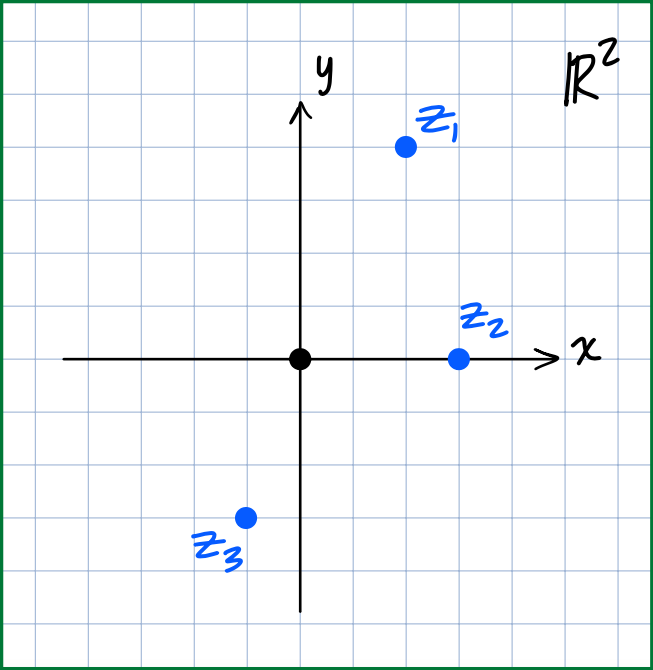
\includegraphics[width=0.3\linewidth]{complexplane}\hspace{4cm} 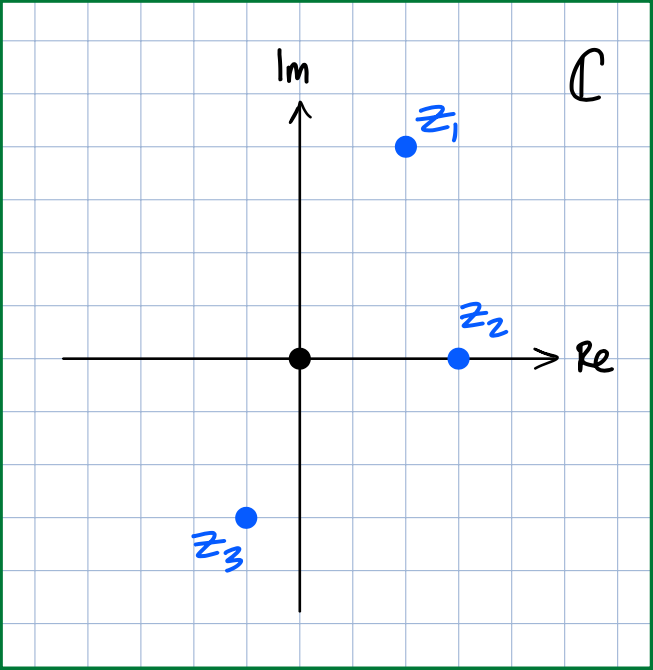
\includegraphics[width=0.3\linewidth]{complexplaneupdated}
\end{center}

\p Note that a point $z\in\COMPLEX$ lies on the $x$-axis if and only if it is real, and lies on the $y$-axis exactly when it is purely imaginary.  On the right, labels are updated accordingly.  $\COMPLEX = \REAL^{2}$ illustrated in this manner is referred to as the \DEF{complex plane}.
\vsp

\p A complex number $z = a + bi$ may also be geometrically represented as an arrow pointing from the origin to the point $(a,b)$ in $\REAL^{2}$, shown on the left.
\vsp

\begin{center}
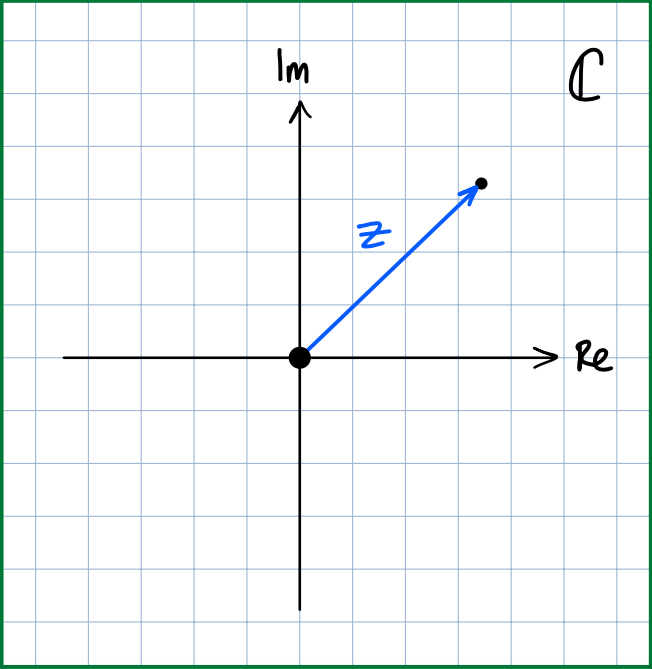
\includegraphics[width=0.3\linewidth]{geometriccomplex}\hspace{4cm} 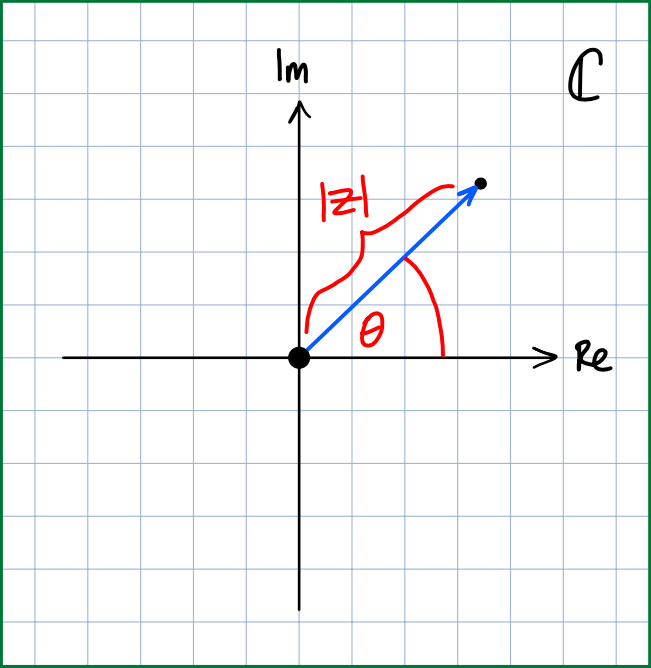
\includegraphics[width=0.3\linewidth]{geometriccomplexlabelled}
\end{center}

\p Any such arrow has length given by the complex modulus of $z$, and forms an angle of inclination, measured counter-clockwise from the positive half of the real axis, shown on the right.

\begin{definition}
An ordered pair $(r,\theta)$ is a polar coordinate representation of $z$ if $r = |z|$ and $\theta$ is the angle of inclination of $z$, measured counter-clockwise from the positive half of the real axis.  In this case $\theta$ is called an \DEF{argument} of $z$.
\end{definition}

\note If $(r,\theta)$ is a polar coordinate representation of a complex number $z$, the Pythagorean Theorem forces real and imaginary parts of $z$ to be given by
\begin{center}
$\RE{z} = r\cos(\theta)$ and $\IM{z} = r\sin(\theta)$.
\end{center}
It follows that $z = r\cos(\theta) + ir\sin(\theta) = r(\cos(\theta) + i\sin(\theta)) = re^{i\theta}$, which is referred to as the \DEF{polar form} of $z$.
\vsp

\observation If $z_{1} = r_{1}e^{i\theta_{1}}$ and $z_{2} = r_{2}e^{i\theta_{2}}$ are written in polar form, then
\begin{center}
$\ds{z_{1}z_{2} = \left(r_{1}e^{i\theta_{1}}\right)\left(r_{2}e^{i\theta_{2}}\right) = (r_{1}r_{2})e^{i\theta_{1} + i\theta_{2}} = r_{1}r_{2}e^{i(\theta_{1} +\theta_{2})}}$
\end{center}
and
\begin{center}
$\ds{z_{1}/z_{2} = \frac{r_{1}e^{i\theta_{1}}}{r_{2}e^{i\theta_{2}}} = \left(\frac{r_{1}}{r_{2}}\right)e^{i\theta_{1} - i\theta_{2}} = \left(\frac{r_{1}}{r_{2}}\right)e^{i(\theta_{1} - \theta_{2})}}$.
\end{center}
\vsp

\p Consequently, to multiply complex numbers in polar form, we \emph{multiply their lengths and add their arguments}.  To divide them, we \emph{divide their lengths, and subtract their arguments}.  This is helpful to make use of when computing powers.  Indeed if $z = re^{i\theta}$ is in polar form and $n\geq 0$, then
\begin{center}
$z^{n} = \left(re^{i\theta}\right)^{n} = r^{n}\left(e^{i\theta}\right)^{n} = r^{n}e^{n(i\theta)} = r^{n}e^{i(n\theta)}$.
\end{center}
\vsp

\p Combining this with Euler's Formula in the special case when $r = 1$, we get the following.
\vsp

\begin{theorem}[DeMoivre's Formula] $(\cos(\theta) + i\sin(\theta))^{n} = \cos(n\theta) + i\sin(n\theta)$
\end{theorem}

\examples
\begin{enumerate}[(a)]
\item Let $z_{1} = 1 + i$ and $z_{2}  = \sqrt{3} - i$.  Find $z_{1}z_{2}$ and $z_{1}/z_{2}$ in polar form.
\item Find $(1 + i)^{16}$.
\end{enumerate}

\subsection{$\ARG{z}$ and $\PARG{z}$}

\p Note that the argument of a complex number is not unique!  For example, in polar form, $1 + i$ may be written as both $\sqrt{2}e^{i(\pi/4)}$ and $\sqrt{2}e^{i(9\pi/4)}$.  So both $\pi/4$ and $9\pi/4$ are arguments for $1 + i$.  More generally, if $\theta$ is an argument for $z\in\COMPLEX$, then so is $\theta + 2\pi k$ for any $k\in \INTEGER$.
\vsp

\notation For any $z\in\COMPLEX$ with argument $\theta$, we may capture all of its arguments with the notation
\begin{center}
$\ARG{z} = \theta + 2\pi k$
\end{center}
where it is understood that $k$ varies over the set of integers.
\vsp

\fact For any $\theta\in\REAL$, there exists a unique $k^{\star}\in\INTEGER$ such that $\theta + 2\pi k^{\star}\in (-\pi, \pi]$.  In this case $\theta + 2\pi k^{\star}$ is called the \DEF{principle argument} of $z$, and is denoted by $\PARG{z}$.
\vsp

\examples
\begin{enumerate}[(a)]
\item For $z = 1 + i$, $\ARG{z} = \pi/4 + 2\pi k$, and $\PARG{z} = \pi/4$.
\item $\PARG{e^{i(5\pi/3)}} = -2\pi/3$.
\end{enumerate}

\begin{exercise} is $Arg(z_1z_2) = Arg(z_1) + Arg(z_2)$?
\end{exercise}

\subsection{Roots of Unity}\label{rootsofunitysection}

\p So far, positive and negative exponents have been defined for complex numbers, but what about rational exponents?  In the case of real numbers, we define
\begin{center}
$x^{m/n} = \sqrt[n]{x^{m}} = \left(\sqrt[n]{x}\right)^{m}$,
\end{center}
whenever $\GCD{m,n} = 1$ and either $x\geq 0$ or $n$ is odd.
\vsp

\p But this takes advantage $n$th roots, which have not yet been defined for complex numbers.  This notion must first be extended to $\COMPLEX$.  But this is no simple matter, since in $\REAL$ for example, there are two fourth roots of $1$: namely $1$ and $-1$.  This is traditionally resolved by defining $\sqrt[4]{1}$ to be the \emph{positive} fourth root of $1$, and then using the notation $\pm \sqrt[4]{1}$ to describe both of the fourth roots of $1$.
\vsp

\p But in $\COMPLEX$, $1$, $-1$, $i$ and $-i$ are \emph{all} fourth roots of $1$!  A new method must be developed to capture all of these roots.
\vsp

\begin{definition}
Let $n\geq 1$.  A complex number $\xi$ is said to be an \DEF{$n$th root of unity} if $\xi^{n} = 1$.
\end{definition}

\example The fourth roots of unity are the complex numbers $1, -1, i$, and $i$.
\vsp

\p For a general $n\geq 1$, it is easier to construct an $n$th root of unity when polar form is considered.
\vsp

\remarks ~\label{rootsofunity}
\begin{enumerate}[(1)]
\item For any integer $n\geq 1$, if $\xi = e^{i(2\pi/n)}$, it may be seen that
\begin{center}
$\xi^{n} = \left(e^{i(2\pi/n)}\right)^{n} = e^{n[i(2\pi/n)]} = e^{i(2\pi)} = 1$.
\end{center}
\p Hence $\zeta = e^{i(2\pi/n)} = \cos(2\pi/n) + i\sin(2\pi/n)$ is an $n$th root of unity.
\item For any $k\in\INTEGER$, $\xi^{k}$ is also an $n$th root of unity.  Indeed we may compute
\begin{center}
$\left(\xi^{k}\right)^{n} = \left(\xi^{n}\right)^{k} = 1^{k} = 1$.
\end{center}
\item The $n$ distinct $n$th roots of unity are given by $\zeta^{k} = e^{i(2\pi k/n)}$, where $k\in\INTEGER$ with $0\leq k < n$.
\end{enumerate}

\example Find all of the eighth roots of unity.

\begin{definition} Let $n\geq 1$.  A complex number $\omega\in\COMPLEX$ is a \DEF{primitive $n$th root of unity} if $\omega^{n} = 1$ and $\omega^{k}\neq 1$ whenever $0 < k < n$.
\end{definition}

\p classify all $n$th roots of unity: if $\omega$ is primitive, then the set of $n$th roots of unity is given by $\SET{\omega^{k}:k=0,1,\dots,n-1}$

\p when is $\omega^{k}$ primitive? when $\GCD{n,k} = 1$

\p solutions to $z^{n} = z_{0} = re^{i\theta}$ are found by taking $r^{1/n}e^{i(\theta/n)}$ and multiplying it by all the different roots of unity

\p -quadratic formula

\section{Congruence in $\INTEGER$ and Modular Arithmetic}\label{congruencechapter}

\subsection{Congruence and Congruence Classes}

\begin{definition}\label{congruenceoperations}
Let $a,b,n\in\INTEGER$ with $n > 0$.  We say that $a$ is \DEF{congruent to $b$ modulo $n$} if $n|b-a$.
\end{definition}

\notation In this case we write $a\equiv b$ (mod $n$), or $a\overset{n}{\equiv}b$.  Otherwise we write $a\not\equiv b$ (mod $n$), or $a\not\overset{n}{\equiv}b$.

\example $9\overset{2}{\equiv}5$ and $9\overset{4}\equiv{5}$ but $9\not\overset{2}{\equiv}5$.

\begin{theorem}\label{congruenceproperties}Let $n\in\INTEGER$ with $n > 0$.
\begin{enumerate}[(1)]
\item $a\overset{n}{\equiv} a$ for any $a\in\INTEGER$.
\item If $a,b\in\INTEGER$ such that $a\overset{n}{\equiv} b$, then $b\overset{n}{\equiv} a$.
\item If $a,b,c\in\INTEGER$ such that $a\overset{n}{\equiv} b$ and $b\overset{n}{\equiv} c$, then $a\overset{n}{\equiv} c$.
\end{enumerate}
\end{theorem}
%
\begin{proof}~
\begin{enumerate}[(1)]
\item For any $a\in\INTEGER$, we have $n|a-a$, since $a-a = 0$.  Hence $a\overset{n}{\equiv} a$.
\item For any $a,b\in\INTEGER$, if $a\overset{n}{\equiv} b$, then $n|b-a$.  Hence $n|a-b$, so $b\overset{n}{\equiv} a$.
\item For any $a,b,c\in\INTEGER$, if $a\overset{n}{\equiv} b$ and $b\overset{n}{\equiv} c$, then $n$ divides both $b-a$ and $c-b$.  It follows that $n$ also divides $c-a = (c-b) + (b-a)$.  Hence $a\overset{n}{\equiv} c$.\hfill \qedhere
\end{enumerate}
\end{proof}
%
\begin{theorem}\label{congruencereplacement}
If $a,b,c,d\in\INTEGER$ such that $a\overset{n}{\equiv} b$ and $c\overset{n}{\equiv} d$, then $a + c\overset{n}{\equiv} b + d$ and $ac\overset{n}{\equiv} bd$.
\end{theorem}
%
\begin{proof}
By assumption, $n|b-a$ and $n|d-c$.  It follows that
\begin{center}
$(b+d) - (a+c) = (b-a) + (d-c)$
\end{center}
and
\begin{center}
$bd - ac = bd - ad + ad - ac = d(b-a) + a(d-c)$.
\end{center}
are both divisible by $n$.  Hence $a + c\overset{n}{\equiv} b + d$ and $ac\overset{n}{\equiv} bd$.
\end{proof}
\vsp

\p In particular, if $a,b\in\INTEGER$ such that $a\overset{n}{\equiv} b$, then for any $c\in\INTEGER$, $a + c\overset{n}{\equiv} b + c$ and $ac\overset{n}{\equiv} bc$ for any $c\in\INTEGER$.

\begin{example}
Find all solutions to the congruence $2x\overset{5}{\equiv} 3$.
\end{example}

\solution Note that $5|2x - 3$ whenever there exists $s\in\INTEGER$ such that $2x - 3 = 5s$.  In other words, the congruence is satisfied whenever
\begin{center}
$\ds{x = \frac{5s + 3}{2}}$
\end{center}
for some integer $s\in\INTEGER$.
\vsp

\begin{exercises} \phantom{ }
\begin{enumerate}[(1)]
\item Find all solutions to the congruence $3x\overset{7}{\equiv} 4$.
\item Which of the following congruences have solutions?
\begin{enumerate}[(a)]
\item $x^{2}\overset{3}{\equiv} 1$
\item $x^{2}\overset{7}{\equiv} 2$
\item $x^{2}\overset{11}{\equiv} 3$
\end{enumerate}
\item Let $a,b,n\in\INTEGER$ with $n > 0$.  Prove that if $a\overset{n}{\equiv}b$, then $a^2 + b^2\overset{n^2}{\equiv}2ab$.
\item Suppose $a,b\in\INTEGER$ such that $a\overset{p}{\equiv}b$ for every prime $p$.  Prove that $a = b$.
\end{enumerate}
\end{exercises}
%
\begin{definition}\label{congruenceclassmodndefn}
Let $a,n\in\INTEGER$ with $n > 0$.  The \DEF{congruence class of $a$ modulo $n$} is defined by
\begin{center}
$[a] = \SET{b\in\INTEGER : a\overset{n}{\equiv}b} = \SET{a + kn:k\in\INTEGER}$.
\end{center}
\end{definition}
%
\begin{example}
If $n = 5$, then
\begin{itemize}[\ ]
\item $[0] = \SET{0 + 5k:k\in\INTEGER} = \SET{5k:k\in\INTEGER}$
\item $[1] = \SET{1 + 5k:k\in\INTEGER} = \SET{1 + 5k:k\in\INTEGER}$
\item $[2] = \SET{2 + 5k:k\in\INTEGER} = \SET{2 + 5k:k\in\INTEGER}$
\item $[3] = \SET{3 + 5k:k\in\INTEGER} = \SET{3 + 5k:k\in\INTEGER}$
\item $[4] = \SET{4 + 5k:k\in\INTEGER} = \SET{4 + 5k:k\in\INTEGER}$
\item $[5] = \SET{5 + 5k:k\in\INTEGER} = \SET{5(1 + k):k\in\INTEGER} = \SET{5k:k\in\INTEGER} = [0]$
\end{itemize}
\p In a similar fashion, $[6] = [1]$ and $[7] = [2]$, etc.
\end{example}
%
\begin{theorem}\label{congruenceequalitycriterion}
Let $a,b,n\in\INTEGER$ with $n > 0$.  $a\overset{n}{\equiv}b$ if and only if $[a] = [b]$.
\end{theorem}
%
\begin{proof}
$(\Rightarrow)$ It must be verified that if $a\overset{n}{\equiv}b$, then $[a] = [b]$.

$(\subset)$ Suppose $c\in[a]$.  Then $c\overset{n}{\equiv}a$.  By assumption, $a\overset{n}{\equiv}b$.  Hence by Theorem \ref{congruenceproperties} (3), we must have $c\overset{n}{\equiv}b$, i.e, $c\in[b]$.

$(\supset)$ This direction follows from an identical argument.

$(\Leftarrow)$ Suppose $[a] = [b]$.  By Theorem \ref{congruenceproperties}, $a\overset{n}{\equiv}a$ and hence $a\in [a]$.  It follows that $a\in[b]$ and therefore $a\overset{n}{\equiv}b$, as required.
\end{proof}
%
\begin{corollary}\label{disjointorsame}
For any $a,b,n\in\INTEGER$ with $n > 0$, either $[a] = [b]$ or $[a]\cap [b] = \emptyset$.
\end{corollary}
%
\begin{proof}
Suppose $a,b\in\INTEGER$ with $[a]\cap[b]\neq\emptyset$.  Then choose $c\in[a]\cap[b]$.  It follows that $a\overset{n}{\equiv}c$ and $b\overset{n}{\equiv}c$.  Therefore $a\overset{n}{\equiv}c\overset{n}{\equiv}b$.  By Theorem \ref{congruenceequalitycriterion}, it follows that $[a] = [b]$.
\end{proof}
%
\begin{corollary}\label{elementsofZn}
Let $n\in\INTEGER$ with $n>0$.
\begin{enumerate}[(1)]
\item If $a\in\INTEGER$ and $r$ is the remainder when $a$ is divided by $n$, then $[a] = [r]$.
\item There are exactly $n$ distinct congruence classes modulo $n$, namely $[0], [1], [2],\ldots, [n-1]$.
\end{enumerate}
\end{corollary}
%
\begin{proof}~
\begin{enumerate}[(1)]
\item Use the Division algorithm to write $a = nq + r$ for some $r,n\in\INTEGER$ with $0\leq r < n$.  Since $a - r = nq$, $n|a-r$ and hence $a\overset{n}{\equiv}r$.  Therefore $[a] = [r]$ by Theorem {congruenceequalitycriterion}.
\item First, note that $[0], [1], [2],\ldots, [n-1]$ are all distinct congruence classes.  Indeed if $[i] = [j]$ for some $i,j\in\INTEGER$ with $0\leq i,j < n$, then $i\overset{n}{\equiv}j$ and hence $n|i-j$.  By the way $i$ and $j$ were chosen, we must have $-n+1 < i-j < n-1$.  Since $i-j$ is divisible by $n$, we must have $i-j = 0$, or equivalently, $i=j$.  On the other hand if $a\in\INTEGER$, then by (1) $[a] = [r]$, where $r$ is the remainder of $a$ when divided by $n$.  Since $0\leq r < n-1$, this completes the proof.\qedhere
\end{enumerate}
\end{proof}
%
\begin{definition}
$\ZN$ is the set of all congruence classes modulo $n$.  That is, $\ZN = \SET{[0], [1], [2],\ldots, [n-1]}$.
\end{definition}
%
\begin{exercises}~
\begin{enumerate}
\item Decide whether each of the following statements are true.  If they are true, then prove them.  Otherwise, provide a counter-example.
\begin{enumerate}[(a)]
\item If $a^2\overset{n}{\equiv}b^2$, then either $a\overset{n}{\equiv}b$ or $a\overset{n}{\equiv}-b$.
\item If $p$ is prime and $a^2\overset{p}{\equiv}b^2$, then either $a\overset{p}{\equiv}b$ or $a\overset{p}{\equiv}-b$.
\item If $[a] = [b]$ in $\ZN$, then $\GCD{a,n} = \GCD{b,n}$.
\end{enumerate}
\item If $[a] = [1]$ in $\ZN$, prove that $\GCD{a,n} = 1$.  Demonstrate also that the converse fails to be true in general.
\end{enumerate}
\end{exercises}
%
\subsection{Modular Arithmetic}
\begin{definition}
The \DEF{sum} and \DEF{product} of $[a]$ and $[b]$ in $\ZN$ is given by
\begin{center}
$[a]\oplus [b] = [a + b]$ and $[a]\odot[b] = [ab]$.
\end{center}
\end{definition}
%
\p Note that in order for these operations to be well-defined, it must be the case that the sum and product of two congruence classes do not depend on the representative chosen from the two congruence classes being added or multiplied.  That is, if $[a] = [a']$ and $[b] = [b']$, then $[a+b] = [a' + b']$ and $[ab] = [a'b']$.
\smsp

\p But this is equivalent to the requirement that $a + b\overset{n}{\equiv} a' + b'$ and $ab\overset{n}{\equiv} a'b'$ whenever $a\overset{n}{\equiv} a'$ and $b\overset{n}{\equiv}b'$.  And this follows immediately from Theorem \ref{congruencereplacement}.
%
\begin{example}In $\Z_{5}$, the addition and multiplication tables are shown below.
\vsmsp

\begin{center}
\bgroup
\def\arraystretch{1.5}
\begin{tabular}{c|ccccc}
$\oplus$ & [0] & [1] & [2] & [3] & [4]\\
\hline
$[0]$ & [0] & [1] & [2] & [3] & [4]\\
$[1]$ & [1] & [2] & [3] & [4] & [0]\\
$[2]$ & [2] & [3] & [4] & [0] & [1]\\
$[3]$ & [3] & [4] & [0] & [1] & [2]\\
$[4]$ & [4] & [0] & [1] & [2] & [3]
\end{tabular}
\hspace{3cm}
\begin{tabular}{c|ccccc}
$\odot$ & [0] & [1] & [2] & [3] & [4]\\
\hline
$[0]$ & [0] & [0] & [0] & [0] & [0]\\
$[1]$ & [0] & [1] & [2] & [3] & [4]\\
$[2]$ & [0] & [2] & [4] & [1] & [3]\\
$[3]$ & [0] & [3] & [1] & [4] & [2]\\
$[4]$ & [0] & [4] & [3] & [2] & [1]
\end{tabular}
\egroup
\end{center}
\end{example}
%
\exercise Write out the addition and multiplication tables for $\Z_6$.
\vsp
%
\begin{definition}
A \DEF{relation} on a set $A$ is a subset of $A\times A$.
\end{definition}
\vsp

\notation If $T$ is a relation on a set $A$, and $a,b\in A$ are such that $(a,b)\in T$, then we write $a\sim b$.
\vsp

\begin{definition}
A relation $T$ on a set $A$ is said to be an \DEF{equivalence relation} if the following conditions are met:
\begin{enumerate}[(1)]
\item $a\sim a$, for all $a,\in A$.
\item $a\sim b \Rightarrow b\sim a$, for all $a,b\in A$.
\item $a\sim b$ and $b\sim c \Rightarrow a\sim c$, for all $a,b,c\in A$.
\end{enumerate}
\end{definition}
%
\begin{examples}\label{equivalencerelationexamples}
\begin{enumerate}[(a)]
\item Define the relation $T$ on $\REAL$ by $T = \SET{(x,x):x\in\REAL}\cup \SET{(x,-x):x\in\REAL}$.  Then $(x,y)\in T$ exactly when $x = y$ or $x = -y$.  That is, $x\sim y$ if and only if $|x| = |y|$.
\item $S = \SET{\Big((x,y), (w,z)\Big):x,y,w,z\in\REAL\text{ with }x = y}$ is a relation on $\REAL^{2}$.  In this case, $(x,y)\sim (w,z)$ if and only if $x = w$.
\item Define another relation on $\REAL^{2}$ by $(x,y)\sim (w,z)$ if and only if both $(x,y)$ and $(w,z)$ are the same distance from the origin.
\item Let $A$ be the set of all students in this class.  Define a relation on $A$ by imposing $a\sim b$ whenever $a$ and $b$ were born in the same month.
\item Let $n\in \INTEGER$ with $n > 0$ and define the relation $T = \SET{(a,b):n|b-a}$.  In other words, $a\sim b$ if and only if $a\overset{n}{\equiv}b$.  By Theorem \ref{congruenceproperties}, $T$ is an equivalence relation.  For this reason, equivalence relations may be thought of as a generalization of congruence modulo $n$.
\end{enumerate}
\end{examples}
%
%\begin{definition}
%A partition of a set $A$ is a collection $\mathcal{T}$ of subsets of $A$ with the properties:
%\begin{enumerate}[(1)]
%\item $A = \CUP_{X\in\mathcal{T}} X$ (i.e, for any $x\in A$, there exists $X\in\mathcal{T}$ such that $x\in X$) 
%\item $X_{1}\cap X_{2} = \emptyset$ for any $X_{1}, X_{2}\in\mathcal{T}$.
%\end{enumerate}
%\end{definition}
%
\begin{definition}
If $T$ is an equivalence relation on a set $A$, then for each $a\in A$, then the \DEF{congruence class of $a$} is given by
\begin{center}
$[a] = \SET{b\in A: a\sim b}$
\end{center}
\end{definition}
%
\begin{theorem}
If $T$ is an equivalence relation on a set $A$, then $\SET{[a]:a\in A}$ forms a partition of $A$, i.e. a disjoint collection of subsets of $A$ that cover $A$.
\end{theorem}
%
\begin{proof}
The fact that $\SET{[a]:a\in A}$ covers $A$ is immediate, since for any $a\in A$, we have $a\in [a]$.  To see that congruence classes are disjoint, copy the proof of
Corollary \ref{disjointorsame}.
\end{proof}
%
\begin{examples}
Identify the congruence classes in each of Examples \ref{equivalencerelationexamples}.
\end{examples}
%
\begin{solution}
\begin{enumerate}[(a)]
\item $[0] = \SET{x\in\REAL: 0 = x\text{ or }0 = -x} = \SET{0}$, and for all $x\in \REAL$ with $x\neq 0$, $[x] = \SET{y\in\REAL: x = y\text{ or }x = -y}= {x,-x}$.
\item For each $(x,y)\in\REAL^{2}$, $[(x,y)] = \SET{(w,z)\in\REAL^{2}:x = y}$ is the vertical line through the point $(x,y)$.
\item For each $(x,y)\in\REAL^{2}$, $[(x,y)] = \SET{(w,z)\in\REAL^{2}: \sqrt{x^2 + y^2} = \sqrt{w^2 + z^2}}$, which is the circle centred at the origin which contains the point $(x,y)$.
\item For each student $a\in A$, $[a] = \SET{b\in A:a\text{ and }b\text{ were born in the same month.}}$.
\item $[a] = \SET{b\in\INTEGER:a\sim b} = \SET{b\in\INTEGER: a\overset{n}{\equiv}b} = \SET{a+kn:k\in\INTEGER}$, which is Definition \ref{congruenceclassmodndefn}.
\end{enumerate}
\end{solution}
%
\begin{theorem}  \label{propertiesofZn} Let $n\in\INTEGER$ with $n>0$.  For any $[a], [b], [c]\in\ZN$,
\begin{enumerate}[(1)]
\item $[a] \oplus [b] = [b]\oplus [a]$ \hfill (Commutativity of addition)
\item $[a] \odot [b] = [b]\odot [a]$ \hfill (Commutativity of multiplication)
\item $[a]\oplus ([b]\oplus [c]) = ([a] \oplus [b])\oplus [c]$ \hfill (Associativity of addition)
\item $[a]\odot ([b]\odot [c]) = ([a] \odot [b])\odot [c]$ \hfill (Associativity of multiplication)
\item $[a]\oplus [0] = [a]$ \hfill (Additive Identity)
\item $[a]\odot [1] = [a]$ \hfill (Multiplicative Identity)
\item There exists $[d]\in \ZN$ such that $[a] \oplus [d] = [0]$ \hfill (Additive inverse)
\item $[a]\odot ([b]\oplus [c]) = [a]\odot [b] \oplus [a]\odot [c]$ \hfill (Distributivity)
\end{enumerate}
\end{theorem}
\vsp

%
\p Up until now, $\oplus$ and $\odot$ have been used to denote addition and multiplication of congruence classes in $\ZN$, in order to distinguish these operations from ordinary addition and multiplication of integers.  But it is a standard approach to make this distinction using context alone, and there is no harm in writing the sum and product of $[a],[b]\in \ZN$ as $[a] + [b]$ and $[a]\cdot [b]$, respectively.
\vsp

\p Moreover, unless there is a risk of confusion, the congruence class $[a]\in\ZN$ will simply be denoted $a$.  For example, calculations in $\Z_5$ such as
\begin{center}
$[13] + [11] = [3] + [1] = [4]$
\end{center}
may be abbreviated as
\begin{center}
$13 + 11 = 3 + 1 = 4$.
\end{center}
On a similar note, it is not incorrect to make statements like $17\in\Z_5$ or $-8\in\Z_5$.  But in this case both $17$ and $-8$ are both labels for the same congruence class $[2]\in\Z_5$.
\vsp

\p In this sense, we may think of $\ZN$ as simply the set of all integers, but with the understanding that any two integers that differ by a multiple of $n$ are in fact equal.  We make use of this convention in the following example.
\vsp

%
\begin{example}
Prove that $(a+b)^{5} = a^{5} + b^{5}$ in $\Z_5$.
\end{example}
\begin{solution}
Expanding in the usual way, we get
\begin{center}
$(a + b)^5 = a^{5} + \underbrace{5a^4b}_{=0} + \underbrace{10a^3b^2}_{=0} + \underbrace{10a^2b^3}_{=0} + \underbrace{5ab^4}_{=0} + b^5 = a^5 + b^5$,
\end{center}
where we have used the fact that $5a^4b, 10a^3b^2, 10a^2b^3$, and $5ab^4$ are all multiples of $5$.
\end{solution}
%

\subsection{The Structure of $\Z_p$ when $p$ is Prime}
\p Unless otherwise stated, assume $n\in\INTEGER$ with $n > 0$.  
\begin{definition}
A non-zero $a\in\ZN$ is a \DEF{zero-divisor} if there exists a non-zero $b\in\ZN$ such that $ab = 0$.
\end{definition}
%
\begin{examples}~
\begin{enumerate}[(a)]
\item $\Z_2$ and $\Z_3$ have no zero-divisors.
\item $2\in\Z_4$ is a zero-divisor, since $2\cdot 2 = 4 = 0$.
\item $2,4,6\in\Z_8$ are all zero-divisors, since $2\cdot 4 = 8 = 0$ and $4\cdot 6 = 24 = 0$.
\end{enumerate}
\end{examples}
\vsp

\question What are the zero-divisors of $\ZN$?
\vsp

\begin{theorem}\label{primepnozerodivisors}
$p\in\INTEGER$ is prime if and only if $\Z_p$ has no zero-divisors.
\end{theorem}
%
\begin{proof}\phantom{-}

$(\Rightarrow)$ Suppose $p$ is prime.  If $a,b\in\Z_p$ such that $ab = 0$, then $p|ab$.  Since $p$ is prime, we have $p|a$ or $p|b$.  Hence either $a=0$ or $b=0$.

$(\Leftarrow)$ If $p$ is not prime, then there exists $m,n\in\INTEGER$ with $1\leq m\leq n < p$ such that $p = mn$.  It follows that $p\ndiv m$ and $p\ndiv n$.  Hence $mn = 0$ but $m\neq 0$ and $n\neq 0$.
\end{proof}
%
\begin{theorem}
Let $p$ be prime.  An element $\Z_{p^2}$ is a zero-divisor if and only if it is a non-zero multiple of $p$.
\end{theorem}
%
\begin{proof}\phantom{-}

$(\Leftarrow)$ If $a\in\Z_{p^2}$ is a non-zero multiple of $p$, then $a = kp$ for some $k\in\INTEGER$.  Since $p^2\ndiv p$, $p\neq 0$ and $ap = kp^2 = k(0) = 0$.  Hence $a$ is a zero-divisor.

$(\Rightarrow)$ Suppose $a,b\in\Z_{p^2}$ with $a\neq0$, $b\neq0$, and $ab = 0$.  Then $p^2|ab$, but $p^2\ndiv a$ and $p^2\ndiv b$.  The only way this can be true is if $p|a$ and $p|b$.  Hence both $a$ and $b$ are multiples of $p$.
\end{proof}
\vsp

\begin{examples}\phantom{-}

\begin{enumerate}[(a)]
\item The zero-divisors in $\Z_{25}$ are $5, 10, 15$, and $20$.
\item The zero-divisors in $\Z_9$ are $3$ and $6$.
\end{enumerate}
\end{examples}
%
\begin{definition}
An element $a\in\ZN$ is called a \DEF{unit} if there exists $b\in \ZN$ such that $ab = 1$.  In this case $b$ is called the \DEF{inverse} of $a$ and we write $a^{-1} = b$.
\end{definition}
%
\newpage
%
\begin{example}
The multiplication table for $\Z_6$ is shown below.  
\bgroup
\begin{center}
\def\arraystretch{1.5}
\begin{tabular}{c|cccccc}
$\odot$ & [0] & [1] & [2] & [3] & [4] & [5]\\
\hline
$[0]$ & $[0]$ & $[0]$ & $[0]$ & $[0]$ & $[0]$ & $[0]$\\
$[1]$ & $[0]$ & $[1]$ & $[2]$ & $[3]$ & $[4]$ & $[5]$\\
$[2]$ & $[0]$ & $[2]$ & $[4]$ & $[0]$ & $[2]$ & $[4]$\\
$[3]$ & $[0]$ & $[3]$ & $[0]$ & $[3]$ & $[0]$ & $[3]$\\
$[4]$ & $[0]$ & $[4]$ & $[2]$ & $[0]$ & $[4]$ & $[2]$\\
$[5]$ & $[0]$ & $[5]$ & $[4]$ & $[3]$ & $[2]$ & $[1]$ 
\end{tabular}
\end{center}
\egroup
\p It can be seen that $1$ and $5$ are units, but $0,2,3$, and $4$ are not.
\end{example}

\begin{exercise}\label{zerodivisorcannotbeunitZn} Show that a zero-divisor in $\ZN$ cannot be a unit.\end{exercise}

\begin{example}
$3\in\Z_9$ is not a unit, because it is a zero-divisor.
\end{example}
%
\begin{lemma}\label{gcdunitlemma}
$a\in\ZN$ is a unit if and only if $a$ and $n$ are co-prime.
\end{lemma}
%
\begin{proof}\phantom{-}

$(\Rightarrow)$ If $a$ and $n$ are not co-prime, then let $d>1$ be a common divisor of $a$ and $n$.  It follows that
\begin{center}
$a(n/d) = d(a/d)(n/d) = (a/d)n = 0$
\end{center}
in $\ZN$.  Since $n\ndiv n/d$, $a$ is a zero-divisor and thus cannot be a unit.

$(\Leftarrow)$ If $a$ and $n$ are co-prime, then $\GCD{a,n} = 1$ and we may choose $s,t\in\INTEGER$ satisfying $sa + tn = 1$.  Then $sa\overset{n}{\equiv} 1$ and hence $a$ is a unit with $a^{-1} = s$.
\end{proof}
%
\begin{theorem}\label{Znallunits}
A positive integer $p$ is prime if and only if every non-zero element of $\Z_p$ is a unit.
\end{theorem}
%
\begin{proof}\phantom{-}

$(\Rightarrow)$ Suppose $p$ is prime, and let $a\in\Z_p$ be non-zero.  Then $p\ndiv a$ and hence $\GCD{a,p} = 1$.  By Lemma \ref{gcdunitlemma}, $a$ is a unit.

$(\Leftarrow)$ Suppose every non-zero element of $\Z_p$ is a unit.  Then $\Z_p$ cannot contain a zero-divisor.  By Theorem \ref{primepnozerodivisors}, $p$ is prime.
\end{proof}

\begin{corollary}
Let $a,b\in\ZN$.  If $a$ is a unit, then the equation $ax = b$ has a unique solution in $\ZN$.
\end{corollary}
%
\begin{proof}\phantom{-}

(Existence) Let $a,b\in\ZN$ with $a\neq 0$.  Since $a(a^{-1}b) = (aa^{-1})b = 1b = b$, $x = a^{-1}b$ is a solution.

(Uniqueness) Suppose for a contradiction that $x_{1},x_{2}\in\ZN$ satisfy $ax_{1} = b$ and $ax_{2} = b$ with $x_{1}\neq x_{2}$.  Then $x_{1} - x_{2}\neq 0$, and $a(x_{1} - x_{2}) = ax_{1} - ax_{2} = b - b = 0$.  Hence $a$ is a zero-divisor which is a contradiction, since $a$ is a unit.
\end{proof}
%
\begin{corollary}
Let $p$ be a prime.  For any $a,b\in\Z_p$ with $a\neq 0$, the equation $ax = b$ has a unique solution in $\Z_p$.
\end{corollary}
%
\begin{corollary}
For any $a,b\in\ZN$, if $a$ and $n$ are co-prime, the equation $ax = b$ has a unique solution in $\ZN$.
\end{corollary}
%
\begin{remark}
The inverse of a unit is unique.  That is, if $a\in\ZN$ is a unit with $ab = 1$ and $ac = 1$, then $b=c$.  To see why this is true, compute $b = (ac)b = (ca)b = c(ab) = c\cdot 1 = c$.
\end{remark}
%
\begin{example}
Solve $24x = 5$ in $\Z_{95}$.
\end{example}
\begin{solution}
The Euclidean Algorithm may be used to show that $\GCD{24,95} = 1$ and that $4\cdot 24\nolinebreak + \nolinebreak(-1)95 =\nolinebreak 1$.  Therefore in $\Z_{95}$, $24^{-1} = 4$ and we may compute $x = 24^{-1}\cdot 5 = 4\cdot 5 = 20$.
\end{solution}
%
\begin{theorem}\label{numbersolutionsinZn}
Let $a,b,n\in\INTEGER$ with $n > 1$ and set $d = \GCD{a,n}$.
\begin{enumerate}[(1)]
\item The equation $ax = b$ has solutions in $\ZN$ if and only if $d|b$.
\item If $d|b$, then $ax = b$ has d distinct solutions in $\ZN$.
\end{enumerate}
\end{theorem}
%
\begin{example}
Find all solutions to $18x = 12$ in $\Z_{24}$.
\end{example}
\begin{solution}
Note first that $\GCD{18,12} = 6$, and $6|12$.  Therefore by Theorem \ref{numbersolutionsinZn}, there are $6$ solutions to $18x=12$ in $\Z_{24}$.  To find them, observe that for any $x\in\Z_{24}$,
\begin{align*}
18x = 12\text{ in }\Z_{24} \Leftrightarrow 18x\overset{24}{\equiv}12 \Leftrightarrow 24|18x - 12 &\Leftrightarrow 18x - 12 = 24k\text{ for some }k\in\INTEGER\\
&\Leftrightarrow 3x - 2 = 4k\text{ for some }k\in\INTEGER\\
&\Leftrightarrow 4|3x - 2\\
&\Leftrightarrow 3x\overset{4}{\equiv}2\\
&\Leftrightarrow 3x = 2\text{ in }\Z_{4} 
\end{align*}
Note that $3$ is a unit and is its own inverse in $\Z_4$ since $3\cdot 3 = 9 = 1$ in $\Z_4$.  Hence in $\Z_4$, the equation $3x=2$ is equivalent to $x = 2$.  Of all the possible values of $x$ in the set
\begin{center}
$Z_{24} = \SET{0,1,2,3,4,5,6,7,8,9,10,11,12,13,14,15,16,17,18,19,20,21,22,23}$,
\end{center}
the ones that satisfy $x = 2$ in $\Z_4$ are $2,6,10,14,18$, and $22$.  These are the solutions we seek.
\end{solution}
%
\section{Rings}
\subsection{Binary Operations}
%
\begin{definition}
A \DEF{binary operation} on a set $S$ is a function $*:S\times S\to S$.  In this case, the pair $(S,*)$ is called a \DEF{binary algebraic structure}.
\end{definition}

\notation For $a,b\in S$, we denote $*(a,b) = a * b$.

\begin{remark}
Instead of using the phrase \emph{$(S,*)$ is a binary algebraic structure}, we often say \emph{$S$ is a binary algebraic structure under $*$}.  And if the operation $*$ is clear from context, we further abbreviate the statement to simply say that \emph{$S$ is a binary algebraic structure}.
\end{remark}

\begin{examples}\label{basexamples}~

\begin{enumerate}[(a)]
\item Addition $+$ and multiplication $\cdot$ are binary operations on $\Z$.  Hence $(\Z,+)$ and $(\Z,*)$ are binary algebraic structures.
\item For an integer $n > 0$, addition $\oplus$ and multiplication $\odot$ from Definition \ref{congruenceoperations} are binary operations on $\ZN$.  Hence $(\ZN,\oplus)$ and $(\Z_{n},\odot)$ are both binary algebraic structures.
%\item $\Z$ is a binary algebraic structure under the operation $*:\Z\times\Z\to\Z$ defined by $a*b = \MIN{a,b}$.  For example, $3*5 = \MIN{3,5} = 3$.
\item Let $M(\REAL)$ denote the set of all matrices with real entries.  Matrix addition $+$ is not a binary operation on $M(\REAL)$, since it is not defined on all of $M(\REAL)\times M(\REAL)$.  For example,
\begin{center}
$\MATRIX{rr}{1 & 3\\2 & 4} + \MATRIX{rr}{1 & 0\\0 & 1\\2 & 1}$
\end{center}
is not defined.
\item Let $M_{2}(\REAL)$ denote the set of all $2\BY 2$ matrices with real entries.  $M_{2}(\REAL)$ is a binary algebraic structure under both matrix addition and matrix multiplication.
\item The set $F(\REAL)$ of all functions $f:\REAL\to\REAL$ is a binary algebraic structure under function composition.
\item \label{dihedralgroup} Consider the set $D_3 = \SET{r_0,r_1,r_2,p_1,p_2,p_3}$ of all possible permutations (illustrated below) of an equilateral triangle that may be achieved through rotations and flips, \emph{in such a way that the triangle occupies exactly the same space before and after the transformation}.

\begin{center}
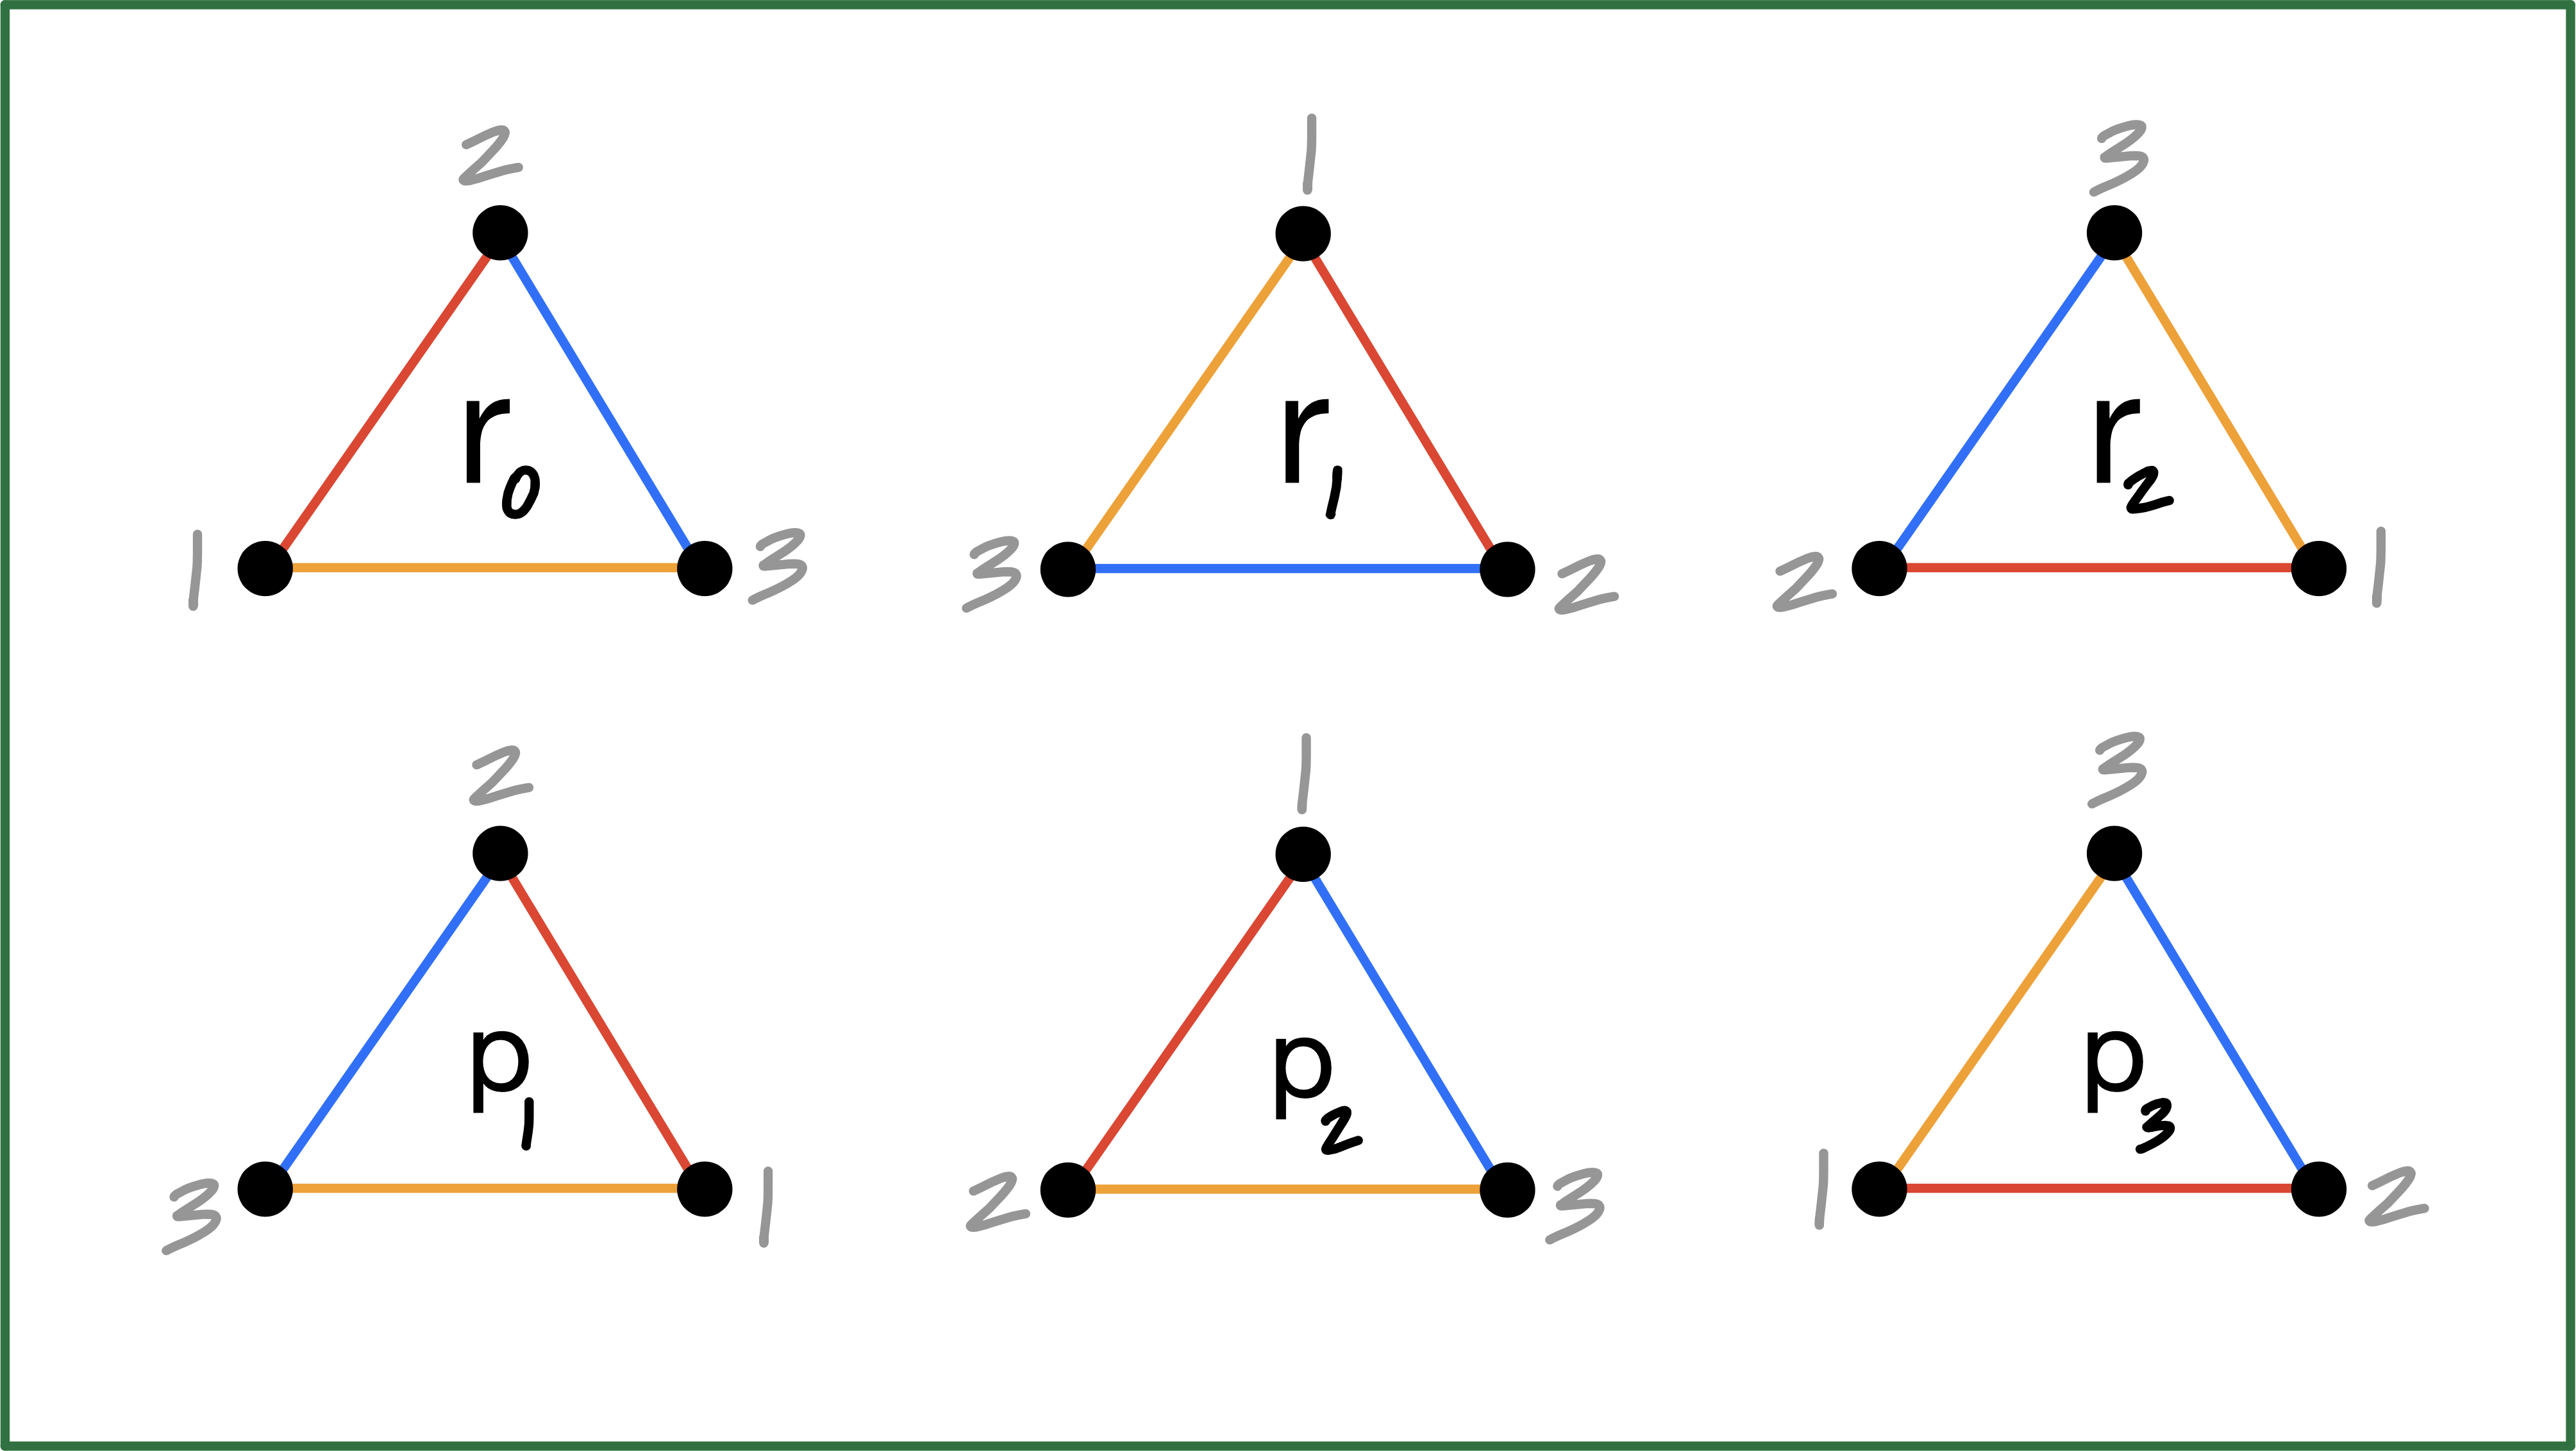
\includegraphics[width=0.5\linewidth]{permutationsoftriangle}
\end{center}

\p Think of the elements of $D_3$ as transformations of the \emph{default} or \emph{neutral} triangle $r_{0}$.  In particular,
\begin{align*}
r_0 &= \text{ clockwise rotation by }0^{\circ}\\
r_1 &= \text{ clockwise rotation by }120^{\circ}\\
r_2 &= \text{ clockwise rotation by }240^{\circ}\\
p_1 &= \text{ flip of the edge connecting vertices }1\text{ and }3\\
p_2 &= \text{ flip of the edge connecting vertices }1\text{ and }2\\
p_3 &= \text{ flip of the edge connecting vertices }2\text{ and }3
\end{align*}
\p Define the following product on $D_{3}$ as follows.  To multiply two elements $x,y\in D_3$, identify the flip or rotation that corresponds to $y$, and then perform it on $x$.  The result is assigned to the product $xy$.  For example,
\begin{center}
$r_{1}r_{1} = r_{2}$ and $r_{1}p_{2} = p_{3}$.
\end{center}
\p The complete multiplication table is given by
\bgroup
\begin{center}
\def\arraystretch{1.5}
\begin{tabular}{c|cccccc}
 & $r_{0}$ & $r_{1}$ & $r_{2}$ & $p_{1}$ & $p_{2}$ & $p_{3}$\\
\hline
$r_{0}$ & $r_{0}$ & $r_{1}$ & $r_{2}$ & $p_{1}$ & $p_{2}$ & $p_{3}$\\
$r_{1}$ & $r_{1}$ & $r_{2}$ & $r_{0}$ & $p_{3}$ & $p_{1}$ & $p_{2}$\\
$r_{2}$ & $r_{2}$ & $r_{0}$ & $r_{1}$ & $p_{2}$ & $p_{3}$ & $p_{1}$\\
$p_{1}$ & $p_{1}$ & $p_{2}$ & $p_{3}$ & $r_{0}$ & $r_{1}$ & $r_{2}$\\
$p_{2}$ & $p_{2}$ & $p_{3}$ & $p_{1}$ & $r_{2}$ & $r_{0}$ &$r_{1}$\\
$p_{3}$ & $p_{3}$ & $p_{1}$ & $p_{2}$ & $r_{1}$ & $r_{2}$ & $r_{0}$
\end{tabular}
\end{center}
\egroup
\p This product turns $D_{3}$ into a binary algebraic structure known as the \DEF{Dihedral Group on $3$ elements}, which may be generalized to $D_n$ for any $n\geq 3$.  This is studied in more detail in Math 3220.  
\end{enumerate}
\end{examples}
%
\begin{definition}
Let $(S,*)$ be a binary algebraic structure.  A subset $H\subset S$ is \DEF{closed under *} if $a*b\in H$ whenever $a,b\in H$.  In this case $\left(H,*\restrict{H\times H}\right)$ is also a binary algebraic structure, and is called a \DEF{sub-structure} of $(S,*)$.
\end{definition}
%
\terminology If the operation $*$ is clear from context, we may simply say that $H$ is a sub-structure of $S$, or that $H$ inherits an algebraic structure from $S$.
%
\begin{examples}~
\begin{enumerate}[(a)]
\item $R^{*} = \SET{x\in\REAL:x\neq 0}\subset \REAL$ is not closed under addition $+$, since $-1,1\in\REAL^{*}$ but $-1 + 1 = 0\notin \REAL^{*}$.  But $R^{*}$ is closed under multiplication, since if $x,y\in\REAL$ are both non-zero, then so is their product.  Hence $\REAL^{*}$ is a (multiplicative) sub-structure of $\REAL$.
\item The set $H = \SET{n^2:n\in\Z}\subset\Z$ is closed under multiplication.  Indeed if $x,y\in H$, then $x = m^2$ and $y=n^2$ for some $m,n\in\Z$.  So $xy = m^2n^2 = (mn)^2$, which is an element of $H$.  But $H$ is not closed under addition since, for example, $1 = 1^2\in H$ and $4 = 2^2\in H$, but $1 + 4 = 5\notin H$.
\end{enumerate}
%
\begin{definition}
A binary operation $*$ on a set $S$ is
\begin{itemize}
\item \DEF{commutative} if $a*b = b*a$ for all $a,b\in S$, and
\item \DEF{associative} if $a*(b*c) = (a*b)*c$ for all $a,b,c\in S$.
\end{itemize}
\end{definition}
\end{examples}
%
\p {\color{blue}TODO: examples, $\Z$ is commutative but $D_3$ is not}\\
\p {\color{blue}TODO: add comment about associative propertes and its connection to defining multiples $na$ and powers $a^n$}
%
\subsection{Isomorphic Binary Structures}

\recall If $X$ and $Y$ are any sets, a map $f:X\to Y$ is said to be
\begin{itemize}
\item \DEF{injective} or \DEF{one-to-one} if whenever $f(x_{1}) = f(x_{2})$, we have $x_{1} = x_{2}$.
\item \DEF{surjective} or \DEF{onto} if for all $y\in Y$, there exists $x\in X$ such that $f(x) = y$.
\end{itemize}
%
\begin{definition}
Let $(S,*)$ and $(S',*')$ be binary algebraic structures.  A bijection $\varphi:S\to S'$ is an \DEF{isomorphism} if $\varphi(a*b) = \varphi(a)*'\varphi(b)$ for all $a,b\in S$.  In this case we say that $(S,*)$ and $(S',*')$ are isomorphic.
\end{definition}
%
\begin{example}\label{firstisomorphismexample}
Let $S = \SET{a,b,c}$ and $S' = \SET{1,2,3}$ be binary algebraic structures under the operations $*$ and $*'$ respectively defined by the following tables:
\begin{center}
\bgroup
\begin{center}
\def\arraystretch{1.5}
\begin{tabular}{c|ccc}
$*$ & $a$ & $b$ & $c$\\
\hline
$a$ & $b$ & $a$ & $c$\\
$b$ & $a$ & $c$ & $b$\\
$c$ & $c$ & $b$ & $a$\\
\end{tabular}
\hspace{3cm}
\begin{tabular}{c|ccc}
$*'$ & $1$ & $2$ & $3$\\
\hline
$1$ & $2$ & $1$ & $3$\\
$2$ & $1$ & $3$ & $2$\\
$3$ & $3$ & $2$ & $1$\\
\end{tabular}
\end{center}
\egroup
\end{center}
\p A close examination of these tables results in the conclusion that the only difference between the binary structures $(S,*)$ and $(S', *')$ is the way the elements are labelled.  If we define $\varphi:S\to S'$ by
\begin{center}
$\varphi(a) = 1, \varphi(b) = 2$, and $\varphi(c) = 3$
\end{center}
it may be checked that $\varphi$ is an isomorphism.  For example
\begin{center}
$\varphi(a*b) = \varphi(a) = 1 = 1*' 2 = \varphi(a)*'\varphi(b)$.
\end{center}
\p But it must also be verified that $\varphi(a*c) = \varphi(a)*'\varphi(c)$ and $\varphi(b*c) = \varphi(b)*'\varphi(c)$.  But even still there are other products to consider!  Only after checking that $\varphi(a*a) = \varphi(a)*'\varphi(a), \ \ \varphi(b*b) = \varphi(b)*'\varphi(b)$, and $\varphi(c*c) = \varphi(c)*'\varphi(c)$, may we finally conclude that $\varphi$ is an isomorphism.  These checks are left to you as an exercise.
\end{example}
%
\begin{exercise}
The set $2\Z := \SET{2n:n\in\Z} = \SET{0, \pm 2, \pm 4,\ldots}$ of even integers is a binary algebraic structure under addition.  Prove that $(\Z,+)$ is isomorphic to $(2\Z,+)$.
\end{exercise}
%
\notation For $a,n\in\Z$ with $n\neq 0$, let $a\text{ mod }n$ denote the remainder when $a$ is divided by $n$.  For example, $15\text{ mod }4 = 3$ and $8\text{ mod }2 = 0$.
%
\begin{examples}~
\begin{enumerate}[(a)]
\item Let $n>0$ be an integer, and recall that in Definition \ref{congruenceoperations}, the set $\ZN = \SET{[a]:a\in\INTEGER}$ of congruence classes modulo $n$ was introduced and equipped with addition and multiplication operations defined by
\begin{center}
$[a]\oplus [b] = [a + b]$ and $[a]\odot [b] = [ab]$, for all $[a],[b]\in\ZN$.
\end{center}
\p Note that $(\ZN,\oplus)$ and $(\ZN,\odot)$ are both binary algebraic structures.
\vsp

\p Consider now the set $\overline{\Z}_{n} = \SET{0,1,2,\ldots, n-1}$, which is also a binary algebraic structure under either of the addition $+_{n}$ and multiplication $\cdot_{n}$ operations defined by
\begin{center}
$a+_{n}b = (a + b)\text{ mod }n$,
\end{center}
and
\begin{center}
$a\cdot_{n}b = (ab)\text{ mod }n$, for all $a,b\in\overline{\Z}_{n}$.
\end{center}

\p The differences between $\overline{\Z}_{n}$ and the $\ZN$ are merely cosmetic!  Indeed define $\varphi:\overline{\Z}_{n}\to \Z_{n}$ by $\varphi(a) = [a]$ for all $a \in \overline{\Z}_{n}$.  By Corollary \ref{elementsofZn}, $\varphi$ is a bijection.  Moreover, for any $a,b\in\overline{\Z}_{n}$, we have 
\begin{center}
$\varphi(a+_nb) = \varphi\big((a+b)\text{ mod }n\big) = [(a+b)\text{ mod }n] = [a+b] = [a]\oplus [b] = \varphi(a)\oplus\varphi(b)$,
\end{center}
and
\begin{center}
$\varphi(a\cdot_nb) = \varphi\big((ab)\text{ mod }n\big) = [(ab)\text{ mod }n] = [ab] = [a]\odot [b] = \varphi(a)\odot\varphi(b)$.
\end{center}
%
\p Hence $(\ZN,\oplus)$ is isomorphic to $(\overline{\Z}_n,+_n)$ and $(\ZN,\odot)$ is isomorphic to $(\overline{\Z}_n,\odot_n)$.  From now on, we will ignore the distinction between the sets $\overline{\Z}_n$ and $\ZN$ and simply write $\ZN$ to refer to whichever one is more convenient to work with in the moment.
%
\item The set $\REAL^{+} = \SET{x\in\REAL:x>0}$ is a binary algebraic structure under multiplication.  It may be seen that $(\REAL^{+},\cdot)$ is isomorphic to $(\REAL, +)$ since the map $\varphi:\REAL\to\REAL^{+}$ defined by $\varphi(x) = e^{x}$ is a bijection, and $\varphi(x+y) = e^{x + y} = e^xe^{y} = \varphi(x)\varphi(y)$, for any $x,y\in\REAL$.
%
\item For any integer $n>0$, the set $U_{n} = \SET{z\in\COMPLEX:z^n = 1}$ of $n$th roots of unity is a binary algebraic structure under multiplication, since if $z_{1},z_{2}\in U_{n}$, we must have $z_{1}^n = 1$ and $z_{2}^n = 1$.  Hence $z_{1}z_{2}\in U_n$ since $(z_{1}z_{2})^n = z_{1}^nz_{2}^n = 1\cdot 1 = 1$.  It turns out that $(U_{n},\cdot)$ is isomorphic to $(\ZN,+)$!
\vsp

\p To see why this is the case, recall the observation made in Remarks \ref{rootsofunity} that
\begin{center}
$U_{n} = \SET{\xi^{k}:k=0,1,2\ldots, n-1}$,
\end{center}
where $\xi = e^{i(2\pi/n)} = \cos(2\pi/n) + i\sin(2\pi/n)$.  Define $\varphi:U_{n}\to\ZN$ by $\varphi(\xi^k) = k$.  It is immediate that $\varphi$ is a bijection, and for any $\xi^{k_1},\zeta^{k_2}\in U_n$ we have
\begin{center}
$\varphi(\zeta^{k_1}\zeta^{k_2}) = \varphi(\xi^{k_1+k_2}) = k_1+k_2 = \varphi(\xi^{k_1}) + \varphi(\xi^{k_1})$.
\end{center}
\end{enumerate}
\end{examples}
%
\begin{lemma}\label{selfsquarelemma}
Suppose $(S,*)$ and $(S',*')$ are isomorphic binary algebraic structures, and that there exists a unique $x\in S$ such that $x*x = x$.  Prove that there exists a unique $y'\in S'$ such that $y'*'y' = y'$.
\end{lemma}
%
\begin{proof}\phantom{-}

\p (Existence) By assumption, there exists an isomorphism $\varphi:S\to S'$.  Take $y' = \varphi(x)$ and check that $y'*y' = \varphi(x)*'\varphi(x) = \varphi(x*x) = \varphi(x) = y'$.
\vsp

\p (Uniqueness) Suppose for a contradiction that there exists $y_{1}',y_{2}'\in S'$ with $y_{1}'\neq y_{2}'$ such that $y_{1}'*'y_{1}' = y_{1}'$ and $y_{2}'*'y_{2}' = y_{2}'$.  Then set $x_{1} = \varphi^{-1}(y_{1}')$ and $x_{2} = \varphi^{-1}(y_{2}')$ and note that
\begin{center}
$x_{1}*x_{1} = \varphi^{-1}\big(\varphi(x_1*x_1\big) = \varphi^{-1}\big(\varphi(x_1)*'\varphi(x_1)\big) = \varphi^{-1}\big(y_{1}'*'y_{1}'\big) = \varphi^{-1}(y_{1}') = x_{1}$
\end{center}
and similarly
\begin{center}
$x_{2}*x_{2} = \varphi^{-1}\big(\varphi(x_2*x_2\big) = \varphi^{-1}\big(\varphi(x_2)*'\varphi(x_2)\big) = \varphi^{-1}\big(y_{2}'*'y_{2}'\big) = \varphi^{-1}(y_{2}') = x_{2}$.
\end{center}
Since $\varphi$ is a bijection and $y_{1}'\neq y_{2}'$, we must have $x_{1}\neq x_{2}$, this is a contradiction.
\end{proof}
%
\begin{theorem}
$(\Z,+)$ and $(\Z,\cdot)$ are not isomorphic.
\end{theorem}
%
\begin{proof}
The equation $x + x = x$, has only one integer solution, namely $x = 0$.  But both $0$ and $1$ are integer solutions to the equation $x\cdot x = x$.  Therefore the result follows by Lemma \ref{selfsquarelemma}.
\end{proof}
%
\begin{definition}
Let $(S,*)$ be a binary algebraic structure.  $e\in S$ is an \DEF{identity element} for $*$ if $e*x = x$ and $x*e = x$ for all $x\in S$.
\end{definition}
%
\begin{examples}~
\begin{enumerate}[(a)]
\item In $(\Z,+)$, $0$ is the identity element.
\item In $(\REAL,\cdot)$, $1$ is the identity element.
\item In $D_3$, $r_{0}$ is the identity element (see Example \ref{basexamples} \ref{dihedralgroup}).
\item In $M_{2}(\REAL)$, $\MATRIX{rr}{1 & 0\\0 & 1}$ is the identity element.
\item The binary algebraic structure $(S,*)$ from Example \ref{firstisomorphismexample} has no identity element.
\end{enumerate}
\end{examples}
%
\begin{remark}\label{uniqueidentities}
A binary algebraic structure $(S,*)$ can have at most one identity element $e$, for if $e'\in S$ is also an identity element, then $e = e*e' = e'$.
\end{remark}
%
\begin{exercise}
Suppose $(S,*)$ and $(S',*')$ are two isomorphic binary algebraic structures.  Prove that if $S$ has an identity element for $*$, that $S'$ has an identity element for $*'$.
\end{exercise}

\subsection{Definition and Examples of Rings}

\begin{definition}\label{ringdefinition}
A \DEF{ring} is a set $R$ with two binary operations $+$ and $\cdot$ satisfying the following properties.
\begin{enumerate}[(1)]
\item $a + b = b + a$, for all $a,b\in R$.
\item $a + (b + c) = (a + b) + c$, for all $a,b,c\in R$.
\item There exists $0_{R}\in R$ such that $a + 0_{R} = a$ for all $a\in R$.\label{additiveidentity}
\item For every $a\in R$, there exists $b\in R$ such that $a + b = 0_{R}$.\label{additiveinverse}
\item $a\cdot(b\cdot c) = (a\cdot b)\cdot c$, for all $a,b,c\in R$.
\item $a\cdot(b + c) = a\cdot b + a\cdot c$, for all $a,b,c\in R$.
\item $(a + b)\cdot c = a\cdot c + b\cdot c$, for all $a,b,c\in R$.\label{rightdistributivity}
\end{enumerate}
\end{definition}
%
\begin{remarks}~
\begin{enumerate}[(1)]
\item The element $0_{R}$ whose existence was postulated in property \ref{additiveidentity} is referred to as the \DEF{additive identity} or \DEF{zero element} of $R$.  This element is unique.  Indeed, similar to the comments made in in Remark \ref{uniqueidentities}, if $0_{R}'\in R$ is another additive identity, then $0_{R} = 0_{R} + 0_{R}' = 0_{R}'$.  When there is no risk of confusion, we drop the subscript and simply denote it by $0$.

\item The element $b$ mentioned in property \ref{additiveinverse} is called the \DEF{additive inverse} of $a$, and is typically denoted by $-a$.  It is also unique, since if $b$ and $b'$ satisfy $a + b = 0$ and $a + b' = 0$, then
\begin{center}
$b = b + 0 = b + (a + b') = (b + a) + b' = (a + b) + b' = 0 + b' = b'$.
\end{center}
\item While subtraction was not explicitly mentioned in Definition \ref{ringdefinition}, we may define it over a ring $R$ by
\begin{center}
$a - b = a + (-b)$, for all $a,b\in R$.
\end{center}
\item As usual, the concatenation $ab$ is often used to represent the product $a\cdot b$ of $a,b\in R$.
\item It follows from the properties listed in Definition \ref{ringdefinition} that $0a = 0$ for any $a\in R$.  Indeed by \ref{rightdistributivity}, we have
\begin{center}
$0a = (0 + 0)a = 0a + 0a$.
\end{center}
It follows that $0a = 0a + 0 = 0a + (0a - 0a) = (0a + 0a) - 0a = 0a - 0a = 0$.
\item Formally speaking, a ring is defined to be a triple $(R,+,\cdot)$, where $(R,+)$ and $(R,\cdot)$ are both binary algebraic structures satisfying the properties listed in Definition \ref{ringdefinition}.  But usually we will casually refer to the set $R$ itself as a ring, with the understanding that it must come equipped with the operations $+$ and $\cdot$.
\end{enumerate}
\end{remarks}
%
\begin{exercises}\label{ringpropertyexercises} Prove the following statements about a ring $R$.
\begin{enumerate}[(a)]
\item $a(b-c) = ab - ac$ and $(a-b)c = ac - bc$ for all $a,b,c\in R$.
\item $-(-a) = a$ for all $a\in R$.
\item $a(-b) = -(ab) = (-a)b$ for all $a,b\in R$.\label{negativeproduct}
\item $-(a+b) = -a - b$ for all $a,b\in R$.
\item $-(a-b) = b-a$ for all $a,b\in R$.
\item $(-a)(-b) = ab$ for all $a,b\in R$.
\end{enumerate}
\end{exercises}
%
\p In particular, a consequence of Exercise \ref{ringpropertyexercises} \ref{negativeproduct} that $-a = (-1)a$ for any $a\in R$.
\vsp

\terminology
\begin{itemize}
\item If $a\cdot b = b\cdot a$ for all $a,b\in R$, then $R$ is said to be \DEF{commutative}.
\item A ring $R$ is said to be \DEF{unital} or a \DEF{ring with identity} if there exists $1_{R}\in R$ such that $1_{R}\cdot a = a$ and $a\cdot 1_{R} = a$ for all $a\in R$.  This element $1_{R}$ is called the \DEF{multiplicative identity} or \DEF{unity} of $R$, and may be denoted as $1$, whenever there is no risk of confusion.
\end{itemize}
%
\begin{examples}\label{ringexamples}~
\begin{enumerate}[(a)]
\item $\Z, \RATIONAL, \REAL$ and $\COMPLEX$, equipped with the standard addition and multiplication operations are all commutative unital rings.
\item Whenever $n\in\Z$ with $n > 0$, $\ZN$ is a commutative unital ring by Theorem \ref{propertiesofZn}.
\item\label{Rsquared} $\REAL^{2} = \SET{(a,b):a,b\in\REAL}$ is a commutative ring with addition $+$ and multiplication $\cdot$ defined by
\begin{center}
$(a_1,b_1) + (a_2,b_2) = (a_1 + a_2,b_1 + b_2)$ and $(a_1,b_1) \cdot (a_2,b_2) = (a_1a_2,b_1b_2)$
\end{center}
for all $(a_1,b_1), (a_2,b_2)\in\REAL^{2}$.  Moreover, $\REAL^{2}$ is unital with identity $1_{\REAL^{2}} = (1,1)$.
\item The set $M_{2}(\REAL) = \SET{\MATRIX{rr}{a & b\\c&d}:a,b,c,d\in\REAL}$ of all $2\BY 2$ matrices with real entries is a ring.

\p Addition and multiplication are defined using the rules
\begin{center}
$\MATRIX{rr}{a_1 & b_1\\c_1 & d_1} + \MATRIX{rr}{a_2 & b_2\\c_2 & d_2} = \MATRIX{cc}{a_1 + a_2 & b_1 + b_2\\c_1 + c_2& d_1 + d_2}$
\end{center}
and
\begin{center}
$\MATRIX{rr}{a_1 & b_1\\c_1 & d_1}\MATRIX{rr}{a_2 & b_2\\c_2 & d_2} = \MATRIX{cc}{a_1a_2 + b_1b_2 & a_1c_2 + b_1d_2\\c_1a_2 + d_1b_2 & c_1b_2 + d_1d_2}$,
\end{center}
\p $M_{2}(\REAL)$ is not commutative, since
\begin{center}
$\MATRIX{rr}{1 & 1\\-1 & 1}\MATRIX{rr}{1 & 1\\2 & 1} = \MATRIX{rr}{3 & 2\\1 & 0}$
\end{center}
but
\begin{center}
$\MATRIX{rr}{1 & 1\\2 & 1}\MATRIX{rr}{1 & 1\\-1 & 1} = \MATRIX{rr}{0 & 2\\ 1 & 3}$,
\end{center}
\p but it is unital with multiplicative identity given by $1_{M_{2}(\REAL)} = \MATRIX{rr}{1 & 0\\0 & 1}$.
\item The set $F(\REAL)$ of all functions $f:\REAL\to\REAL$ is a commutative ring, when equipped with point-wise addition and multiplication:
\begin{center}
$(f+g)(x) = f(x) + g(x)$
\end{center}
and
\begin{center}
$(fg)(x) = f(x)g(x)$,
\end{center}
for all $f,g\in F(\REAL)$.  $F(\REAL)$ is also unital with $1_{F(\REAL)}$ equal to the constant function which is identically $1$ on $\REAL$.
\item The singleton $R = \SET{0}$ is a ring, with addition and multiplication operations defined by $0 + 0 = 0$ and $0\cdot 0 = 0$.  And it may be odd to say so, but $R$ is in fact unital, since $0$ satisfies the definition of both the additive and multiplicative identity!  In this case $R$ is called the \DEF{zero ring}, or \DEF{null ring} and is sometimes written as $R = 0$.  Any other ring is said to be \DEF{non-zero}.
\end{enumerate}
\end{examples}
%
\begin{exercise}
Show that $(F(\REAL), +, \circ)$ fails to be a ring when $\oplus$ represents point-wise addition and $\circ$ corresponds to function composition.
\end{exercise}
%
\begin{definition}
Let $R$ be a ring.  A subset $S\subset R$ is a \DEF{subring} of $R$ if it is a ring when equipped with the operations inherited from $R$.
\end{definition}
%
\begin{example}
$\Z$ is a subring of $\RATIONAL$, $\RATIONAL$ is a subring of $\REAL$, and $\REAL$ is a subring of $\COMPLEX$.
\end{example}
%
\begin{remarks}~
\begin{enumerate}[(a)]
\item Note that if $R$ is any ring, then both $R$ and the zero ring are automatically subrings of $R$.  Any other subring of $R$ is said to be \DEF{proper}.
\item A subring $S$ of a commutative ring $R$ is commutative.  Since if
\begin{center}
$ab = ba$ for all $a,b\in R$,
\end{center}
then the weaker statement
\begin{center}
$ab = ba$ for all $a,b\in S$
\end{center}
must be true as well, as the elements of $S$ are among those in $R$.
\end{enumerate}
\end{remarks}
%
\begin{theorem}[Subring Criterion]
If $R$ is a ring, then any subset $S\subset R$ is a subring of $R$ if:
\begin{enumerate}[(1)]
\item $a+b\in S$ and $ab\in S$ whenever $a,b\in S$
\item $0_{R}\in S$
\item $-a\in S$ whenever $a\in S$.
\end{enumerate}
\end{theorem}
%
\begin{proof}
We directly verify that any subset $S\subset R$ satsifying $(1)-(3)$ above, automatically satisfies all of the properties listed in Definition \ref{ringdefinition}.
\begin{enumerate}[(1)]
\item Since $a + b = b + a$ for every $a,b\in R$, this equation certainly holds for all $a,b\in S$.
\item Similarly, $a + (b +c)  = (a + b) + c$ holds for every $a,b,c\in R$, so it must hold for every $a,b,c\in S$.
\item The existence of $0_{S}\in S$ such that $0_{S} + a = a$ for all $a\in S$ is guaranteed by assumption (2) which says that $0_R\in S$.  Simply take $0_S = 0_R$.
\item For each $a\in S$, assumption (3) guarantees that $-a\in S$.  Hence the requirement for additive inverses is immediately satisfied.
\item Since $a\cdot(b\cdot c) = (a\cdot b)\cdot c$ for every $a,b,c\in R$, it must also hold for every $a,b,c\in S$.
\item $a\cdot (b + c) = a\cdot b + a\cdot c$ for every $a,b,c\in S$, because the same equation holds for all $a,b,c\in R$.
\item Similarly, $(a + b)\cdot c = a\cdot c + b\cdot c$ for every $a,b,c\in R$ so it must hold for every $a,b,c\in S$.\qedhere
\end{enumerate}
\end{proof}
\smsp

%
\begin{example}\label{abnegativebasubring}
The set
\begin{center}
$S = \SET{\MATRIX{rr}{a & b\\-b & a}:a,b,\in\REAL}$
\end{center}
is a subring of $M_{2}(\REAL)$, which may be proved using the Subring Criterion.  First, suppose $A,B\in S$ and choose $a_{1},b_{1},a_{2},b_{2}\in\REAL$ such that
\begin{center}
$A = \MATRIX{rr}{a_{1} & b_{1}\\-b_{1} & a_{1}}$ and $B = \MATRIX{rr}{a_{2} & b_{2}\\-b_{2} & a_{2}}$.
\end{center}
It follows that
\begin{center}
$A + B = \MATRIX{rr}{a_{1} & b_{1}\\-b_{1} & a_{1}} + \MATRIX{rr}{a_{2} & b_{2}\\-b_{2} & a_{2}} =  \MATRIX{rr}{\phantom{-(}a_{1} + a_{2}\phantom{)}& b_{1} + b_{2}\\-(b_{1} + b_{2}) & a_{1} + a_{2}}\in S$
\end{center}
and
\vsp

\begin{adjustwidth}{-100pt}{-100pt}
\begin{center}
$AB = \MATRIX{rr}{a_{1} & b_{1}\\-b_{1} & a_{1}}\MATRIX{rr}{a_{2} & b_{2}\\-b_{2} & a_{2}} = \MATRIX{cc}{\phantom{-}a_1a_2 - b_1b_2 & \phantom{-}a_1b_2 + b_1a_2\\-b_1a_2-a_1b_2 & -b_1b_2 + a_1a_2} = \MATRIX{cc}{\phantom{-(}a_1a_2 - b_1b_2\phantom{)} & a_1b_2 + b_1a_2\\-(a_1b_2 + b_1a_2) & a_1a_2 - b_1b_2}\in S$.
\end{center}
\end{adjustwidth}
\vsp

\p To see that (2) holds, note that the additive identity in $M_2(\REAL)$ is (the \DEF{zero matrix}) given by
\begin{center}
$O = \MATRIX{rr}{0 & 0\\0 & 0}$,
\end{center}
which is also in $S$ since
\begin{center}
$O = \MATRIX{rr}{0 & 0\\0 & 0} = \MATRIX{rr}{a & b\\-b & a}$, where $a = 0$ and $b = 0$.
\end{center}
\p Finally, if $A = \MATRIX{rr}{a & b\\-b & a}\in S$, then $-A = \MATRIX{rr}{-a & -b\\b & -a} = \MATRIX{cc}{-a & -b\\-(-b) & -a}\in S$, which verifies $(3)$.
\end{example}

\begin{exercise}\label{zadjoinroottwosubringofreal}
Show that $\Z[\sqrt{2}] = \SET{a + b\sqrt{2}:a,b\in\Z}$ is a subring of $\REAL$.
\end{exercise}
%
\begin{definition}
Let $R$ and $S$ be rings.  The \DEF{Cartesian product} of $R$ and $S$ is defined as
\begin{center}
$R\times S = \SET{(r,s):r\in R,s\in S}$,
\end{center}
equipped with addition and multiplication defined by
\begin{center}
$(r_1,s_1) + (r_2,s_2) = (r_1 + r_2,s_1 + s_2)$ and $(r_1,s_1)\cdot(r_2,s_2) = (r_1r_2,s_1s_2)$
\end{center}
for all $(r_1,s_1),(r_2,s_2)\in R\times S$.
\end{definition}
%
\begin{remarks}~
\begin{enumerate}[(1)]
\item The additive identity for $R\times S$ is given by $0_{R\times S} = (0_{R},0_{S})$.
\item The additive inverse of any $(r,s)\in R\times S$ is given by $-(r,s) = (-r,-s)$.
\item If $R$ and $S$ are unital, then so is $R\times S$, with $1_{R\times S} = (1_{R},1_{S})$.
\end{enumerate}
\end{remarks}
%
\begin{example}~
%\item In Examples \ref{ringexamples} \ref{Rsquared} we defined the ring $\REAL^{2}$, which is no different than the Cartesian product $\REAL\times\REAL$.
Consider the the Cartesian product
\begin{center}
$\Z_{5}\times M_{2}(\REAL) =\SET{(n,A):n\in\Z_5, A\in M_{2}(\REAL)}$,
\end{center}
and choose two elements in particular, say
\begin{center}
$\left(4, \MATRIX{rr}{1 & 1\\3 & 5}\right)$ and $\left(2, \MATRIX{rr}{-1  & 1\\0 & 1}\right)$.
\end{center}
We may add them by computing
\begin{center}
$\left(4, \MATRIX{rr}{1 & 1\\3 & 5}\right) + \left(2, \MATRIX{rr}{-1  & 1\\0 & 1}\right) = \left(4 + 2, \MATRIX{rr}{1 & 1\\3 & 5} + \MATRIX{rr}{-1  & 1\\0 & 1}\right) = \left(1, \MATRIX{rr}{0 & 2\\3 & 6}\right)$
\end{center}
or multiply them as
\begin{center}
$\left(4, \MATRIX{rr}{1 & 1\\3 & 5}\right)\cdot \left(2, \MATRIX{rr}{-1  & 1\\0 & 1}\right) = \left(4\cdot 2, \MATRIX{rr}{1 & 1\\3 & 5}\MATRIX{rr}{-1  & 1\\0 & 1}\right) = \left(3, \MATRIX{rr}{-1 & 2\\-3 & 8}\right)$.
\end{center}
\p Since $\Z_{5}$ and $M_{2}(\REAL)$ are both unital, so is $\Z_{5}\times M_{2\BY 2}(\REAL)$ with identity $\left(1,\MATRIX{rr}{1 & 0\\0 & 1}\right)$.
\end{example}
%
\subsection{Integral Domains and Fields}
%
\begin{definition}
Let $R$ be a ring.  An element $a\in R$ is a \DEF{zero divisor} if there exists a non-zero $b\in R$ such that $ab = 0$.  In this case $b$ is also a \DEF{zero divisor}.
\end{definition}
%
\begin{definition}
A non-zero commutative unital ring is an \DEF{integral domain} if it has no zero divisors.
\end{definition}
%
\begin{examples}~
\begin{enumerate}[(a)]
\item $\Z, \RATIONAL, \REAL$, and $\COMPLEX$ are all integral domains.
\item By Theorem \ref{primepnozerodivisors}, if $p$ is prime, $\Z_p$ is an integral domain.
\item $\Z_{30}$ is not an integral domain.  Indeed $2$ and $15$ are zero divisors since $2\cdot 15 = 30 = 0$ in $\Z_{30}$.
\vsmsp

\p More generally, any composite integer $n>1$ can be factored as $n = mk$ for some integers $m$ and $k$ with $1 < m\leq k < n$.  It follows that $m$ and $k$ are zero divisors since $mk = n = 0$ in $\ZN$, so $\ZN$ contains zero divisors and is hence not an integral domain.
\item $M_{2}(\REAL)$ is not an integral domain, since $\MATRIX{rr}{1 & 0\\0 & 0}\MATRIX{rr}{0 & 0\\0 & 1} = \MATRIX{rr}{0 & 0\\0 & 0}$.
\end{enumerate}
\end{examples}
%
\begin{exercise}
Let $R$ and $S$ be rings.  Prove that the Cartesian product $R\times S$ is an integral domain if and only if both $R$ and $S$ are integral domains.
\end{exercise}
%
\begin{definition}
Let $R$ be a unital ring (not necessarily commutative).  An element $a\in R$ is a \DEF{unit} if there exists $b\in R$ such that $ab = 1$ and $ba = 1$.  In this case, we call $b$ the \DEF{multiplicative inverse} of $a$.
\end{definition}
%
\begin{remark}
Multiplicative inverses are unique!  Indeed if $b_{1},b_{2}\in R$ both satisfy $ab_{1} = ab_{2} = 1$ and $b_{1}a = b_{2}a = 1$, then we must have
\begin{center}
$b_1 = 1\cdot b_1 = (b_2a)b_1 = b_2(ab_1) = b_2\cdot 1 = b_2$.
\end{center}
\end{remark}
%
\begin{examples}~
\begin{enumerate}[(a)]
\item In $\Z$, the only units are $1$ and $-1$.
\item By Lemma \ref{gcdunitlemma}, $a\in \ZN$ is a unit if and only if $\GCD{a,n} = 1$.
\item In $\RATIONAL$ and $\REAL$, every non-zero element is a unit.
\item By Theorem \ref{Znallunits}, every non-zero element of $\Z_p$ is a unit whenever $p$ is prime.
\item In $M_{2}(\REAL)$, the units are the matrices with non-zero determinants.  That is, the matrices of the form
\begin{center}
$\MATRIX{rr}{a & b\\c & d}$
\end{center}
satisfying $ad - bc \neq 0$.
\end{enumerate}
\end{examples}
%
\begin{exercise}
Let $R$ be a ring.  Is the set $U=\SET{a\in R:a\text{ is a unit}}$ a subring of $R$?
\end{exercise}
%
\begin{lemma}\label{unitscantbezerodivisors}
If $R$ is a unital ring, and then no unit can be be a zero-divisor.
\end{lemma}
%
\begin{proof}
If $a\in R$ is a unit and a zero-divisor, we could choose non-zero $b\in R$ such that $ab = 0$.  But then
\begin{center}
$b = (a^{-1}a)b = a^{-1}(ab) = a^{-1}\cdot 0 = 0$,
\end{center}
which is a contradiction.
\end{proof}
%
\begin{definition}
A \DEF{field} $F$ is a non-zero commutative unital ring with the property that every non-zero element $a\in F$ is a unit.
\end{definition}
%
\begin{examples}~
\begin{enumerate}[(a)]
\item $\RATIONAL, \REAL$, and $\COMPLEX$ are all fields.
\item $\Z$ is not a field, since $2$ has no inverse.
\item In a manner similar to Exercise \ref{zadjoinroottwosubringofreal}, it may be checked that $\RATIONAL[\sqrt{2}] = \SET{a + b\sqrt{2}:a,b\in\RATIONAL}$ is a subring of $\REAL$, and in fact it is a field!  Certainly $\RATIONAL[\sqrt{2}]$ is commutative as it is a subring of $\REAL$, and it is unital, since $1 = 1 + 0\sqrt{2}\in\RATIONAL[\sqrt{2}]$.  Finally, we verify that any non-zero $a+b\sqrt{2}\in \RATIONAL[\sqrt{2}]$ is a unit.  Of course in $\REAL$ we may compute
\begin{center}
$(\ds{a + b\sqrt{2})\left(\frac{1}{a + b\sqrt{2}}\right) = 1}$.
\end{center}
So all that need be checked is that $\dfrac{1}{a + b\sqrt{2}}\in \RATIONAL[\sqrt{2}]$, and indeed
\begin{center}
$\ds{\frac{1}{a + b\sqrt{2}} = \frac{1}{a + b\sqrt{2}}\cdot\frac{a - b\sqrt{2}}{a - b\sqrt{2}} = \frac{a - b\sqrt{2}}{a^2 + 2b^2} = \underbrace{\frac{a}{a^2 + 2b^2}}_{\in\RATIONAL} + \underbrace{\frac{-b}{a^2 + 2b^2}}_{\in\RATIONAL}\sqrt{2}\in\RATIONAL[\sqrt{2}]}$.
\end{center}
\end{enumerate}
\end{examples}
%
\begin{theorem}\label{fieldisdomain}
Every field is an integral domain.
\end{theorem}
%
\begin{proof}
If $F$ is a field, then it is already a non-zero commutative unital ring.  So all that is left to show is that $F$ has no zero-divisors.  But every non-zero $a\in F$ is a unit.  So by Lemma \ref{unitscantbezerodivisors}, $F$ cannot be a zero-divisor.
\end{proof}
%
\begin{remark}
Note that the converse of Theorem \ref{fieldisdomain} is false, with $\Z$ serving as a counter-example.
\end{remark}
%
\begin{theorem}
A finite integral domain $D$ is a field.
\end{theorem}
%
\begin{proof}
Let $D^{*} = \SET{a\in D:a\neq 0}$ and define for each $a\in D^*$ the map $\lambda_{a}:D^{*}\to D^{*}$ by $\lambda_{a}(x) = ax$.  Note that $\lambda_{a}$ is a bijection.  To see injectivity, suppose $\lambda_{a}(x_{1}) = \lambda_{a}(x_{2})$.  It follows that
\begin{center}
$a(x_{1} - x_{2}) = ax_1 - a_x2 =  \lambda_{a}(x_{1}) - \lambda_{a}(x_{2}) = 0$.
\end{center}
Since $a\neq 0$, it cannot be a zero-divisor and hence $x_{1} - x_{2} = 0$, or equivalently, $x_{1} = x_{2}$.  To see surjectivity, suppose for a contradiction that $y\in D^{*}$ such that $\lambda_{a}(x)\neq y$ for all $x\in D^{*}$.  Since $\lambda_{a}$ is injective, the set
\begin{center}
$\lambda_{a}(D^{*}) = \SET{\lambda_{a}(x):x\in D^{*}}$
\end{center}
has the same number of elements as $D^{*}$.  But by assumption $y\notin \lambda_{a}(D^{*})$, so
\begin{center}
$\lambda_{a}(D^{*})\cup \SET{y}$
\end{center}
is a subset of $D^{*}$ with more elements than $D^{*}$.  This is a contradiction.
\vsp

\p Returning to the main claim, since $\lambda_{a}$ is a bijection, $\lambda_{a}(D^{*}) = D^{*}$, which contains $1$.  Hence there exists $x\in D^{*}$ such that $ax = \lambda_{a}(x) = 1$.  It follows that $a$ is a unit, and since $a$ was chosen to be an arbitrary non-zero element of $D$, $D$ must be a field.  
\end{proof}
\vsp

\subsection{Cancellation Properties}

\p When faced with an integer equation such as $x + 3 = y + 3$, we often cancel the $3$'s without hesitation and conclude that $x = y$.  This is usually justified by saying that we are \emph{subtracting $3$} from both sides of the equation, a possibility which generalizes to any ring.

\begin{theorem}[Additive Cancellation]\label{additivecancellation}
If $R$ is a ring, and $a,b,c\in R$ such that
\begin{center}
$a + c = b + c$,
\end{center}
then $a = b$.
\end{theorem}
%
\begin{proof}
If $a + c = b + c$, then $a = a + 0 = a + (c - c) = (a + c) - c = (b + c) - c = b + (c - c) = b+0 = b$.
\end{proof}

\p Similarly, we take it as self-evident that an equation such as $x + 2 = 5$ has a unique solution in $\Z$, namely $x = 5-2 = 3$.  This also generalizes to any ring.
%
\begin{theorem}
Let $R$ be a ring and fix $a,b\in R$.  The equation $a + x = b$ has a unique solution in $R$.
\end{theorem}
%
\begin{proof}~

\p (Existence) Taking $x = b - a$ yields a solution since
\begin{center}
$a + x = a + (b-a) = a + (-a + b) = (a - a) + b = 0 + b = b$.
\end{center}
\p (Uniqueness) If $x_{1},x_{2}\in R$ are two distinct solutions to the equation $a + x = b$ in $R$, then
\begin{center}
$a + x_{1} = b$ and $a + x_{2} = b$.
\end{center}
It follows that $x_{1} - x_{2} = x_{1} - x_{2} + a - a = (a+x_{1}) - (a+x_{2}) = b - b = 0$, and hence $x_{1} = x_{2}$.
\end{proof}
%
\p For our next observation, note that the equation $3x = 10$ does not have a solution in $\Z$, but it does have a (unique) solution in $\RATIONAL$.  This is because $3$ is not a unit in $\Z$, but it is a unit in $\RATIONAL$!  The following theorem generalizes this observation, and also takes the order of multiplication into account.
%
\begin{theorem}\label{unituniquesolution}
Let $R$ be a ring.  If $a\in R$ a unit, then for any $b\in R$, the equations $ax = b$ and $ya = b$ have a unique solution in $R$.
\end{theorem}
%
\begin{proof} We shall prove that the first equation $ax = b$ has a unique solution in $R$, and leave the second equation as an exercise, which is handled in a similar fashion.
\vsp

\p (Existence) It may be checked that $x = a^{-1}b$ is a solution since $ax = a(a^{-1}b) = (a^{-1}a)b = 1\cdot b = b$.
\vsp

\p (Uniqueness) If $x_{1},x_{2}\in R$ are two distinct solutions in $R$, then
\begin{center}
$a(x_{1} - x_{2}) = ax_{1} - ax_{2} = b - b = 0$,
\end{center}
and since $a$ is a unit (and hence not a zero divisor), we must have $x_{1} - x_{2} = 0$, or equivalently, $x_{1} = x_{2}$.
\end{proof}
%
\begin{corollary}
Let $F$ be a field and fix $a,b\in F$ with $a\neq 0$.  The equation $ax = b$ has a unique solution in $F$.
\end{corollary}
\begin{proof}
Since $F$ is a field, $a$ must be a unit in $F$.  Therefore the result follows immediately from Theorem \ref{unituniquesolution}.
\end{proof}

\p When we encounter an integer equation such as $ax = ay$, we conclude without hesitation that $x = y$.  But this does not generalize to any ring.  For example in $\Z_6$ we have $4\cdot 3 = 12 = 0$ and $2\cdot 3 = 6 = 0$.  Hence $4\cdot 3 = 2\cdot 3$ but $4\neq 2$.  This is explained by the fact that $3$ is not a unit in $\Z_6$.
\vsp

\begin{theorem}[Multiplicative Cancellation]
If $R$ is a ring, and $a,b,c\in R$ with $a$ being a unit with $ab = ac$, then we must have $b = c$.
\end{theorem}
%
\begin{proof}
If $ab = ac$, then $b = 1\cdot b = (a^{-1}a)b = a^{-1}(ab) = a^{-1}(ac) = (a^{-1}a)c = 1\cdot c = c$.
\end{proof}
%
\subsection{Ring Homomorphisms}
\begin{definition}
Let $R$ and $S$ be rings.  A map $f:R\to S$ is a homomorphism if
\begin{center}
$f(a+b) = f(a) + f(b)$ and $f(ab) = f(a)f(b)$ for all $a,b\in R$.
\end{center}
\end{definition}
%
{\p \color{blue}TODO: mention homomorphisms of unital rings, which must satisfy $f(1) = 1$, perhaps put this in an exercise}
%
\begin{examples}\label{homomorphismexamples}~
\begin{enumerate}[(a)]
\item If $n$ is a positive integer, then define $f:\Z\to\ZN$ defined by $f(a) = [a]$ for all $a\in\Z$.  It follows from Definition \ref{congruenceoperations} that $f$ is a homomorphism.
\item If $R$ and $S$ are any rings, then the \DEF{zero map} $f:R\to S$, defined by $f(a) = 0_{S}$ for all $a\in R$ is a homomorphism, since
\begin{center}
$f(a + b) = 0 = 0 + 0 = f(a) + f(b)$ and $f(ab) = 0 = 0\cdot 0 = f(a)f(b)$
\end{center}
for any $a,b\in R$.  In this case $f$ is called the \DEF{zero homomorphism}.
\item If $R$ is a ring, and $S\subset R$ is a subring of $R$, then the \DEF{inclusion map} $\iota:S\to R$ defined by $\iota(x) = x$ for all $x\in S$ is a homomorphism.
\item If $R$ is a ring, then the \DEF{identity map} $\text{id}:R\to R$ defined by $\text{id}(x) = x$ for all $x\in R$ is a homomorphism.
\item Let $R_1$ and $R_2$ be rings.  The \DEF{projections}
\begin{center}
$p_{1}:R_1\times R_2\to R_1$ and $p_2:R_1\times R_2\to R_2$,
\end{center}
defined by
\begin{center}
$p_1(x,y) = r$ and $p_2(x,y) = s$ for all $x\in R_1,y\in R_2$,
\end{center}
are homomorphisms.
\item Let $R_1$ and $R_2$ be rings.  The \DEF{embeddings}
\begin{center}
$\iota_1:R_1\to R_1\times R_2$ and $\iota_2:R_2\to R_1\times R_2$,
\end{center}
defined by
\begin{center}
$\iota_1(x) = (x,0)$ and $\iota_2(y) = (0,y)$, for all $x\in R_1,y\in R_2$,
\end{center}
are homomorphisms.
\item Recall that $F(\REAL)$ is a ring under pointwise addition and multiplication.  For any $a\in \REAL$, the map $p_{a}:F(\REAL)\to \REAL$ defined by
\begin{center}
$p_a(f) = f(a)$, for all $f\in F(\REAL)$,
\end{center}
is called the \DEF{point-evaluation map}, and is a homomorphism.
\end{enumerate}
\end{examples}
%
\begin{example}
Define the map $f:\Z\to\Z$ by $f(a) = na$ for all $a\in R$.  Show that $f$ is a homomorphism if and only if $n$ is either $0$ or $1$.
\end{example}
%
\begin{solution}
If $f$ is a homomorphism, then
\begin{center}
$n = f(1) = f(1\cdot 1) = f(1)\cdot f(1) = n\cdot n = n^2$.
\end{center}
Hence $n^2 = n$, which is satisfied if and only if $n = 0$ or $n=1$.
\end{solution}
%
\begin{definition}
Let $R$ and $S$ be rings.  A homomorphism $f:R\to S$ is an \DEF{isomorphism} if it is also a bijection.  In this case we say that $R$ and $S$ are \DEF{isomorphic}.
\end{definition}
%
\begin{examples}~
\begin{enumerate}[(a)]
\item If $n$ is any positive integer, the map $f:\Z\to\ZN$ defined by $f(a) = [a]$ for all $a\in R$ is surjective but not injective.  Indeed $f(0) = [0] = [n] = f(n)$ but $n\neq 0$.
\item The zero map $f:R\to S$ is not injective unless $R$ is the zero ring, and is not surjective unless $S$ is the zero ring.
\item If $S$ is a subring of $R$, the inclusion map $\iota:S\to R$ is injective but not surjective unless $S = R$.
\item For any ring $R$, the identity map $id:R\to R$ is a bijection.  It follows that any ring is isomorphic to itself.
\item If $R_{1}$ and $R_{2}$ are non-zero rings, the projections $p_{1}:R_{1}\times R_{2}\to R_{1}$ and $p_{2}:R_{1}\times R_{2}\to R_{2}$ are surjective but not injective.
\item If $R_{1}$ and $R_{2}$ are non-zero rings, the embeddings $\iota_1:R_1\to R_{1}\times R_{2}$ and $\iota_2:R_2\to R_{1}\times R_{2}$ are injective but not surjective.
\item If $a\in \REAL$, the point-evaluation map $p_{a}:F(\REAL)\to \REAL$ is surjective but not injective.
\end{enumerate}
\end{examples}
%
\begin{exercise}
Recall from Example \ref{abnegativebasubring} where it was verified that
\begin{center}
$S = \SET{\MATRIX{rr}{a & b\\-b&a}}$
\end{center}
is a subring of $M_{2}(\REAL)$.  Prove that $\varphi:S\to\COMPLEX$ defined by
\begin{center}
$\varphi\left(\MATRIX{rr}{a & b\\-b&a}\right) = a + bi$
\end{center}
is an isomorphism.
\end{exercise}
%
\begin{theorem}\label{homomorphismproperties}
Let $R$ and $S$ be rings and let $f:R\to S$ be a homomorphism.
\begin{enumerate}[(1)]
\item $f(0_{R}) = 0_{S}$
\item $f(-a) = -f(a)$ for any $a\in R$.
\item $f(a - b) = f(a) - f(b)$ for any $a,b\in R$.
\item If $R$ is unital and $f$ is surjective, then $S$ is unital and $f(1_{R}) = 1_{S}$.
\item If $u\in R$ is a unit, then $f(u)$ is a unit in $S$ with inverse $f(u^{-1})$.
\end{enumerate}
\end{theorem}
%
\begin{proof}~
\begin{enumerate}[(1)]
\item Note that $f(0_{R}) + 0_{S} = f(0_{R}) = f(0_{R} + 0_{R}) = f(0_{R}) + f(0_{R})$, and hence by Theorem \ref{additivecancellation}, we must have $f(0_{R}) = 0_{S}$.
\item Since $f(a) + f(-a) = f(a + (-a)) = f(0_{R}) = 0_{S}$, it follows that $f(-a) = -f(a)$.
\item $f(a - b) = f(a + (-b)) = f(a) + f(-b) = f(a) - f(b)$.
\item For any $b\in S$, choose $a\in R$ such that $f(a) = b$.  It follows that
\begin{center}
$f(1_{R})b = f(1_{R})f(a) = f(1_{R}a) = f(a) = b$ and $bf(1_{R}) = f(a)f(1_{R}) = f(a1_{R}) = f(a) = b$.
\end{center}
Hence $f(1_{R})$ must be the multiplicative identity of $S$.  That is, $f(1_{R}) = 1_{S}$.
\item If $u\in R$ is a unit, then
\begin{center}
$f(u^{-1})f(u) = f(u^{-1}u) = f(1_{R}) = 1_{S}$ and $f(u)f(u^{-1}) = f(uu^{-1}) = f(1_{R}) = 1_{S}$,
\end{center}
and hence $f(u)^{-1} = f(u^{-1})$.
\end{enumerate}
\end{proof}
%
\p {\color{blue}TODO: talk about how isomorphisms preserve algebraic structures, justifying the following examples}
%
\begin{examples}
\begin{enumerate}[(a)]
\item Is $\Z$ isomorphic to $\ZN$?  No, there cannot be a bijection between $\Z$ and $\ZN$ because $\Z$ is infinite and $\ZN$ is infinite.
\item Is $\Z$ isomorphic to $\RATIONAL$?  No, because $\RATIONAL$ is a field but $\Z$ is not.
\item Is $\RATIONAL$ isomorphic to $\REAL$?  No, because $\RATIONAL$ is countable but $\REAL$ is not.
\end{enumerate}
\end{examples}
\end{document}

